\subsection{\texorpdfstring{\(\mathcal{M}(\mathrm{X};\mathbf{C})\) 中的紧收敛}{M(X; C) 中的紧收敛}}

回顾一下，\(\mathcal{M}(\mathrm{X};\mathbf{C})\) 上的紧收敛拓扑就是在 \(\mathcal{K}(\mathrm{X};\mathbf{C})\) 的紧子集上的一致收敛拓扑。我们把 \(\mathcal{M}(\mathrm{X};\mathbf{C})\) 上在 \(\mathcal{K}(\mathrm{X};\mathbf{C})\) 的严格紧子集（No.~1）上的一致收敛拓扑称为严格紧收敛拓扑。

命题 17. --- 在空间 \(\mathcal{M}(\mathrm{X};\mathbf{C})\) 上，考虑下列诸拓扑：

\(\mathcal{T}_1\) ：关于一个全子集 \(\mathrm{T}\) （\(\mathcal{K}(\mathrm{X};\mathbf{C})\) 的）的逐点收敛拓扑；

\(\mathcal{T}_2\) ：淡拓扑；

\(\mathcal{T}_3\) ：严格紧收敛拓扑；

\(\mathcal{T}_4\) ：紧收敛拓扑。

这些拓扑中的每一个都比其后一个粗。此外：

\begin{enumerate}
\def\labelenumi{(\roman{enumi})}
\item
  对 \(\mathcal{T}_2\) 、 \(\mathcal{T}_3\) 与 \(\mathcal{T}_4\) 而言，有界集是相同的。
\item
  若 \(\mathbf{H}\) 是 \(\mathcal{M}(\mathrm{X};\mathbf{C})\) 的一个淡有界子集，则 \(\mathbf{H}\) 上由 \(\mathcal{T}_1, \mathcal{T}_2, \mathcal{T}_3, \mathcal{T}_4\) 诸拓扑诱导的拓扑是相同的。
\end{enumerate}

\(\mathcal{M}(X;C)\) 的淡有界子集 H 是等度连续的（No.~9, 命题 15），于是第一个断言由 TVS, III, §3, No.~7, 命题 9 得出，第二个断言由 GT, X, §2, No.~4, Th. 1 得出。

回顾一下，当 X 仿紧时，严格紧收敛拓扑与紧收敛拓扑一致（No.~1, 命题 2）。

命题 18. --- 在锥 \(\mathcal{M}_{+}(X)\) 上，由下列诸拓扑诱导的拓扑彼此重合：

\(\mathcal{T}_{1}\) ：关于 \(\mathcal{K}(X;C)\) 的一个在 \(\mathcal{K}(X;C)\) 中稠密且满足性质（P）的线性子空间 V 的逐点收敛拓扑（No.~7, 命题 9）；

\(\mathcal{T}_2\) ：淡拓扑；

\(\mathcal{T}_3\) ：严格紧收敛拓扑。

由于每个滤子都是比它细的诸超滤子之交（GT, I, §6, No.~4, 命题 7），只需证明：若 \(\mathfrak{U}\) 是 \(\mathcal{M}_{+}(\mathrm{X})\) 上的一个超滤子，测度 \(\mu_0\) 是它对拓扑 \(\mathcal{T}_1\) 的极限，则 \(\mu_0\) 也是它对 \(\mathcal{T}_3\) 的极限。设 \(\mathbf{K}\) 是 \(\mathbf{X}\) 的一个紧子集；按假设，存在一个函数 \(h \in \mathrm{V}\) ，它 \(\geqslant 0\) 于 \(\mathbf{X}\) 且取值 \(>0\) 于 \(\mathbf{K}\) ；由此可知每个函数 \(f \in \mathcal{K}(\mathrm{X},\mathrm{K};\mathbf{C})\) 都可写成 \(f = gh\) ，其中 \(g \in \mathcal{K}(\mathrm{X},\mathrm{K};\mathbf{C})\) ，并且若 \(c = \inf_{x \in \mathrm{K}} h(x) > 0\) ，则 \(\| g \| \leqslant c^{-1} \| f \|\) 。按假设，存在一个集 \(\mathrm{H}_0 \in \mathfrak{U}\) ，使得对每个测度 \(\mu \in \mathrm{H}_0\) ，

\[
0 \leqslant \mu (h) \leqslant \mu_ {0} (h) + 1 = b.
\]

因而，对每个函数 \(f \in \mathcal{K}(\mathrm{X};\mathbf{C})\) ，有

\[
| \langle f, h \cdot \mu \rangle | = | \langle h f, \mu \rangle | \leqslant \| f \| \cdot \mu (h) \leqslant b \| f \|
\]

对每个测度 \(\mu\in\mathrm{H}_{0}\) 成立；这就证明：测度 \(h\cdot\mu\) （\(\mu\) 跑遍 \(\mathrm{H}_{0}\) ）所成的集 H 是淡有界的。若 \(\mathfrak{U}_{0}\) 是 \(\mathfrak{U}\) 在 \(\mathrm{H}_{0}\) 上诱导的超滤子，则 \(\mathfrak{U}_{0}\) 在映射 \(\mu\mapsto h\cdot\mu\) 下的像是 H 上某个超滤子 \(\mathfrak{F}\) 的基；又因 H 对严格紧收敛拓扑是相对紧的（命题 17 与 No.~9, 命题 15），故 \(\mathfrak{F}\) 对该拓扑收敛于某个测度 \(\nu_{0}\) 。换言之，对任意 \(\varepsilon>0\) 以及 \(\mathcal{K}(\mathrm{X},\mathrm{K};\mathbf{C})\) 的任意紧子集 L ，存在 \(\mathrm{H}_{0}\) 的一个属于 \(\mathfrak{U}\) 的子集 N ，使得对每个函数 \(g\in\mathrm{L}\) 及属于 N 的任意一对测度 \(\mu,\mu'\) ，有 \(|\langle g,h\cdot\mu\rangle-\langle g,h\cdot\mu'\rangle|\leqslant\varepsilon\) ，即

\[
| \langle g h, \mu \rangle - \langle g h, \mu^ {\prime} \rangle | \leqslant \varepsilon .
\]

而上面我们已经看到，映射 \(g \mapsto gh\) 是 Banach 空间 \(\mathcal{K}(\mathrm{X},\mathrm{K};\mathbf{C})\) 的一个自同构。于是我们已证明 U 是 \(\mathcal{M}_{+}(\mathrm{X})\) 上对严格紧收敛拓扑的 Cauchy 滤子。从而它更是对淡收敛的 Cauchy 滤子，且 No.~9 的命题 14 表明它淡收敛于某个测度 \(\mu_{1}\) ；此外，由于 V 在 \(\mathcal{K}(\mathrm{X};\mathbf{C})\) 中稠密，假设蕴涵 \(\mu_{1} = \mu_{0}\) ；最后，由于 U 是对严格紧收敛拓扑的 Cauchy 滤子，它对该拓扑也收敛于 \(\mu_{0}\) （GT, X, §1, No.~5, 命题 5）。

证毕。

推论. --- 若 X 仿紧，则淡拓扑与紧收敛拓扑在 \(\mathcal{M}_{+}(X)\) 上诱导的拓扑重合。

然而，当 X 不是仿紧的时候，紧收敛拓扑与严格紧收敛拓扑在 \(\mathcal{M}_{+}(X)\) 上诱导的拓扑可能不同（习题 3）。

\section{测度的支集}

\subsection{测度在开集上的限制. 借助局部数据定义测度}

设 X 是一个局部紧空间，Y 是 X 的一个开集。X 的子空间 Y 是局部紧的，并且每个定义在 Y 上、取值于某个拓扑向量空间 E 且具紧支集的连续函数，都可以通过在 \(\complement \mathrm{Y}\) 上取值 0 而连续地延拓到整个 X；于是可以把空间 \(\mathcal{K}(\mathrm{Y};\mathrm{E})\) 以这种方式等同于 \(\mathcal{K}(\mathrm{X};\mathrm{E})\) 中由紧支集含于 Y 的连续函数所构成的线性子空间。若 \(\mu\) 是 X 上的一个测度，则显然 \(\mu\) 在 \(\mathcal{K}(\mathrm{Y};\mathbf{C})\) 上的限制是 Y 上的一个测度，称为 \(\mu\) 在开子空间 Y 上的限制，或 \(\mu\) 在 Y 上诱导的测度，记作 \(\mu|\mathrm{Y}\) 。依据 §1, No.~5 与 No.~6 ， \(|\mu|\) 、 \(\mathcal{R}\mu\) 与 \(\mathcal{I}\mu\) 在 Y 上的限制分别是 \(|\mu|\mathrm{Y}|\) 、 \(\mathcal{R}(\mu|\mathrm{Y})\) 与 \(\mathcal{I}(\mu|\mathrm{Y})\) 。若 \(\mu\) 是实测度，则依据 §1, No.~5 的公式 (8)， \(\mu^{+}\) 与 \(\mu^{-}\) 在 Y 上的限制分别是 \((\mu|\mathrm{Y})^{+}\) 与 \((\mu|\mathrm{Y})^{-}\) 。

立即可见：若 Y 与 Z 是 X 中满足 \(Y \supset Z\) 的两个开集，且 \(\mu|Y\) 与 \(\mu|Z\) 是 \(\mu\) 在 Y 与 Z 上的限制，则 \(\mu|Z\) 也是 \(\mu|Y\) 在局部紧空间 Y 的开子空间 Z 上的限制。

在 Ch. IV, §5, No.~7 中，我们将把这一定义推广到 Y 是 X 的局部紧子空间的情形。

\pandocbounded{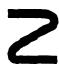
\includegraphics[keepaspectratio]{images/part001_8e0e9629.jpg}}

注意，Y 上的测度未必是 X 上某个测度的限制（参见 Ch. V, §7, No.~2, 命题 3）。

例如，设 Y 是 X = R 中的开区间 {]}0,1{[} ；映射

\[
f \mapsto \int_ {0} ^ {1} \frac {f (x)}{x} d x
\]

是 Y 上的一个测度，因为 \(\mathcal{K}(\mathrm{Y};\mathbf{C})\) 中的每个函数都在 \(\mathbf{R}\) 中 0 的某个邻域上为零。然而这个测度不能延拓为 \(\mathbf{R}\) 上的测度，因为倘若不然，它在函数 \(f\in \mathcal{K}(\mathrm{Y};\mathbf{C})\) （满足 \(\| f\| \leqslant 1\) ）所成之集上的限制将是有界的；而这是不成立的。

不过，我们有下列命题：

命题 1. --- 设 \((\mathrm{Y}_{\alpha})_{\alpha\in\mathrm{A}}\) 是 X 的一个开覆盖，并在每个子空间 \(Y_{\alpha}\) 上给定一个测度 \(\mu_{\alpha}\) ，使得对每个指标对 \((\alpha,\beta)\) ， \(\mu_{\alpha}\) 与 \(\mu_{\beta}\) 在 \(Y_{\alpha}\cap Y_{\beta}\) 上的限制相同。在这些条件下，存在 X 上唯一的测度 \(\mu\) ，使得它在 \(Y_{\alpha}\) 上的限制等于 \(\mu_{\alpha}\) ，对每个指标 \(\alpha\) 均是如此。

首先证明每个函数 \(f \in \mathcal{K}(\mathrm{X};\mathbf{C})\) 都可写成有限和 \(f = \sum_{i} f_{i}\) 的形式，其中对每个函数 \(f_{i} \in \mathcal{K}(\mathrm{X};\mathbf{C})\) ，存在一个指标 \(\alpha_{i}\) 使 \(\operatorname{Supp}(f_{i}) \subset \mathrm{Y}_{\alpha_{i}}\) 。若 \(\mathrm{K} = \operatorname{Supp}(f)\) ，则存在有限个指标 \(\alpha_{i} (1 \leqslant i \leqslant n)\) 使诸 \(\mathrm{Y}_{\alpha_{i}}\) 构成 \(\mathrm{K}\) 的一个覆盖；设 \(h_{i} (1 \leqslant i \leqslant n)\) 是 \(\mathrm{X}\) 到 {[}0,1{]} 中的连续映射，使得 \(h_{i}\) 的支集是紧的且含于 \(\mathrm{Y}_{\alpha_{i}}\) （对 \(1 \leqslant i \leqslant n\) ），并且 \(\sum_{i=1}^{n} h_{i}(x) = 1\) 在 \(\mathrm{K} (\S 1, \text{No. 2, Lemma 1})\) 上成立；函数 \(f_{i} = f h_{i}\) 即合要求。这首先表明：若存在满足要求的测度 \(\mu\) ，则它是唯一的，因为对每个有限和 \(f = \sum_{i=1}^{n} f_{i}\) （其中 \(f_{i} \in \mathcal{K}(\mathrm{Y}_{\alpha_{i}}; \mathbf{C})\) ），必有 \(\mu(f) = \sum_{i=1}^{n} \mu_{\alpha_{i}}(f_{i})\) 。其次，只要证明了下述性质，我们也就证明了存在一个线性形式 \(\mu\) ，它定义在 \(\mathcal{K}(\mathrm{X};\mathbf{C})\) 上，且在每个子空间 \(\mathcal{K}(\mathrm{Y}_{\alpha};\mathbf{C})\) 上的限制为 \(\mu_{\alpha}\) ：若 \((g_{i})_{1 \leqslant i \leqslant m}\) 与 \((h_{j})_{1 \leqslant j \leqslant n}\) 是 \(\mathcal{K}(\mathrm{X};\mathbf{C})\) 中函数的两个有限序列，满足 \(g_{i} \in \mathcal{K}(\mathrm{Y}_{\alpha_{i}}; \mathbf{C})\) 对 \(1 \leqslant i \leqslant m\) 成立， \(h_{j} \in \mathcal{K}(\mathrm{Y}_{\beta_{j}}; \mathbf{C})\) 对 \(1 \leqslant j \leqslant n\) 成立，且

\[
\sum_ {i = 1} ^ {m} g _ {i} (x) = \sum_ {j = 1} ^ {n} h _ {j} (x) = 1
\]

在 K 上成立，则

\[
\sum_ {i = 1} ^ {m} \mu_ {\alpha_ {i}} (f g _ {i}) = \sum_ {j = 1} ^ {n} \mu_ {\beta_ {j}} (f h _ {j}).
\]

现在，

\[
f g _ {i} = \sum_ {j = 1} ^ {n} f g _ {i} h _ {j},
\]

由此得

\[
\sum_ {i = 1} ^ {m} \mu_ {\alpha_ {i}} (f g _ {i}) = \sum_ {i = 1} ^ {m} \sum_ {j = 1} ^ {n} \mu_ {\alpha_ {i}} (f g _ {i} h _ {j}).
\]

同理，

\[
\sum_ {j = 1} ^ {n} \mu_ {\beta_ {j}} (f h _ {j}) = \sum_ {j = 1} ^ {n} \sum_ {i = 1} ^ {m} \mu_ {\beta_ {j}} (f g _ {i} h _ {j}).
\]

但由于 \(fg_{i}h_{j}\) 的支集含于 \(\mathbf{Y}_{\alpha_i}\cap \mathbf{Y}_{\beta_j}\) ，我们有 \(\mu_{\alpha_i}(fg_i h_j) = \mu_{\beta_j}(fg_i h_j)\) ，这就证明了我们的断言。

剩下要说明 \(\mu\) 是 X 上的测度；而 X 的每一点都具有含于某个 \(Y_{\alpha}\) 的紧邻域；因此结论立即由 \(\mu\) 的定义及 §1, No.~3 的命题 6 得出。

推论（局部化原理）. --- 设 \(\mu\) 与 \(\nu\) 是 X 上的两个测度，并设 \((\mathrm{Y}_{\alpha})\) 是 X 的一族开集，使得对每个 \(\alpha\) ， \(Y_{\alpha}\) 上 \(\mu\) 与 \(\nu\) 的限制相等；则 \(\mu\) 与 \(\nu\) 在 \(Y = \bigcup_{\alpha} Y_{\alpha}\) 上的限制相等。

\subsection{测度的支集}

设 \(\mu\) 是局部紧空间 \(X\) 上的一个测度，设 \(\mathfrak{G}\) 是开集 \(U \subset X\) （\(\mu\) 在 \(U\) 上的限制为零）所成的集；由局部化原理（No.~1, 命题 1 的推论）立即可知，若 \(U_0\) 是诸集 \(U \in \mathfrak{G}\) 的并，则 \(U_0\) 本身属于 \(\mathfrak{G}\) ，因而是 \(\mathfrak{G}\) 中最大的开集。

定义 1. --- 设 \(\mu\) 是局部紧空间 \(X\) 上的一个测度，我们把 \(\mu\) 的支集（记作 \(\operatorname{Supp}(\mu)\) ）定义为 \(X\) 中使 \(\mu\) 的限制为零的最大开集的余闭集。

说一点 \(x \in X\) 不属于 \(\mu\) 的支集，意味着存在 x 的一个开邻域 V 使 \(\mu\) 在 V 上的限制为零；因此，说 x 属于 \(\mu\) 的支集，就意味着对 x 的每个邻域 V，存在一个函数 \(f \in \mathcal{K}(X; \mathbf{C})\) ，其支集含于 V，使 \(\mu(f) \neq 0\) 。

例子. --- 1) 为使 X 上的一个测度为零，必须且只须其支集为空集。

\begin{enumerate}
\def\labelenumi{\arabic{enumi})}
\setcounter{enumi}{1}
\item
  \(\mathbf{R}\) 上的 Lebesgue 测度的支集是整条直线 \(\mathbf{R}\) ；因为它是非空的，且在每个平移下不变。
\item
  在区间 \(\mathrm{X} = [0,1]\) （\(\mathbf{R}\) 中）上取一个可数稠密集，把它排成序列 \((a_n)\) ，并设 \(\mu\) 是把质量 \(2^{-n}\) 放在点 \(a_n\) 处（对每个 \(n \geqslant 0\) ）所定义的测度（§1, No.~3, 例 I）。 \(\mu\) 的支集是整个 \(\mathrm{X}\) ；因为设 \(x\) 是 \(\mathrm{X}\) 的任一点， \(\mathrm{V}\) 是 \(x\) 的一个邻域， \(f\) 是一个连续实值函数， \(\geqslant 0\) 于 \(\mathrm{X}\) ，在点 \(x\) 处等于 1，且其支集含于 \(\mathrm{V}\) （§1, No.~2, 引理 1）；\(y \in \mathrm{V}\) （\(f(y) > 0\) ）所成之集在 \(\mathrm{X}\) 中是开集，因而包含某点 \(a_n\) ，于是 \(\mu(f) \geqslant f(a_n)2^{-n} > 0\) 。
\end{enumerate}

命题 2. --- 测度 \(\mu\) 的支集与测度 \(|\mu|\) 的支集相同；若 \(\mu\) 是实测度，则其支集是测度 \(\mu^{+}\) 与 \(\mu^{-}\) 的支集之并。

因为若 \(\mu\) 在某个开集 U 上的限制为零，则 \(|\mu|\) 的限制（相应地， \(\mu^{+}\) 与 \(\mu^{-}\) 的限制，当 \(\mu\) 为实测度时）也为零，反之亦然。

\pandocbounded{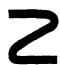
\includegraphics[keepaspectratio]{images/part001_dfbe8ad7.jpg}}

注意， \(\mu^{+}\) 与 \(\mu^{-}\) 的支集可以都非空且相同（参见 Ch. V, § 5, 习题 5）。

命题 3. --- 若 \(\mu\) 与 \(\nu\) 是局部紧空间 X 上满足 \(|\mu| \leqslant |\nu|\) 的两个测度，则 \(\operatorname{Supp}(\mu) \subset \operatorname{Supp}(\nu)\) 。

因为若 \(\nu\) 在某个开集上的限制为零，则 \(\mu\) 的限制也为零。

命题 4. --- 两个测度之和的支集含于其支集之并。

因为若两个测度在某个开集上的限制为零，则其和的限制同样为零。

若 \(\mu\) 与 \(\nu\) 是两个正测度，则 \(\lambda = \mu + \nu\) 的支集等于 \(\mu\) 与 \(\nu\) 的支集之并；因为若 \(x_0\) 是该并中的一点且 V 是 \(x_0\) 的任一邻域，则存在一个连续函数 \(f \geqslant 0\) ，其支集含于 V，且使 \(\mu(f)\) 、 \(\nu(f)\) 两数之一 \(>0\) ；更有甚者， \(\lambda(f) = \mu(f) + \nu(f) > 0\) 。

命题 5. --- 测度 \(\mu\) 在开集 U 上的限制的支集是 \(\mu\) 的支集在 U 上的迹。

由定义，该命题是显然的。

命题 6. --- 局部紧空间 X 上支集含于一个闭集 F 的测度所成之集，是 \(\mathcal{M}(\mathrm{X};\mathbf{C})\) 的一个淡闭线性子空间。

因为它是方程为 \(\mu(f) = 0\) 的淡闭超平面之交，其中 f 跑遍 \(\mathcal{K}(\mathrm{X};\mathbf{C})\) 中支集与 F 不相交的函数所成之集。

设 X 不是紧的：给定一个滤子 \(\Phi\) （在 X 上测度的空间 \(\mathcal{M}(\mathrm{X};\mathbf{C})\) 上），我们说测度 \(\mu\) 的支集沿 \(\Phi\) 退向无穷，如果对 X 的每个紧子集 K，存在一个集 \(M\in\Phi\) ，使得 \(\operatorname{Supp}(\mu)\cap K=\varnothing\) 对每个测度 \(\mu\in M\) 成立。

命题 7. --- 若 \(\Phi\) 是 \(\mathcal{M}(\mathrm{X};\mathbf{C})\) 上的一个滤子，使得测度 \(\mu\) 的支集沿 \(\Phi\) 退向无穷，则 \(\mu\) 关于 \(\Phi\) 淡收敛于 0。

设 \(f\) 是 \(\mathcal{K}(\mathrm{X};\mathbf{C})\) 中的任一函数， \(K\) 是其支集。按假设，存在一个集 \(M \in \Phi\) ，使得对每个测度 \(\mu \in M\) ， \(\operatorname{Supp}(\mu) \cap K = \varnothing\) ；由此得 \(\mu(f) = 0\) 对所有 \(\mu \in M\) 成立，这就证明了该命题。

\subsection{测度支集的刻画}

按定义，若函数 \(f \in \mathcal{K}(\mathrm{X};\mathbf{C})\) 的支集与测度 \(\mu\) 的支集不相交，则 \(\mu(f) = 0\) ；但下述更精确的结果成立：

命题 8. --- 设 \(\mu\) 是局部紧空间 \(X\) 上的一个测度。对每个函数 \(f \in \mathcal{K}(X; \mathbf{C})\) （在 \(\operatorname{Supp}(\mu)\) 上为零），有 \(\mu(f) = 0\) 。

设 \(\mathrm{K} = \operatorname{Supp}(f)\) ， \(\mathrm{S} = \operatorname{Supp}(\mu)\) 。给定一个数 \(\varepsilon > 0\) ，设 \(\mathrm{V}\) 是 \(x \in \mathrm{X}\) （\(|f(x)| < \varepsilon\) ）所成之集；按假设 \(\mathrm{V}\) 是包含 \(\mathrm{S}\) 的开集，因此 \(\complement \mathrm{S}\) 是紧集 \(\complement \mathrm{V}\) 的一个邻域。由此可知，存在一个连续映射 \(h\) ，它把 \(\mathrm{X}\) 映到 {[}0,1{]} 中，在 \(\complement \mathrm{V}\) 上等于 1 且支集含于 \(\complement \mathrm{S}\) （§1, No.~2, 引理 1）。由于 \(fh\) 的支集与 \(\mathrm{S}\) 不相交，故 \(\mu(fh) = 0\) 。另一方面， \(f = fh\) 在 \(\mathrm{K} \cap \complement \mathrm{V}\) 上成立，且 \(|fh| \leqslant |f|\) 在 \(\mathrm{X}\) 上成立，故 \(|f - fh| \leqslant 2\varepsilon\) 在 \(\mathrm{X}\) 上成立（由 \(\mathrm{V}\) 的取法）。最后注意，存在一个数 \(\mathrm{M}_{\mathrm{K}}\) ，使得 \(|\mu(g)| \leqslant \mathrm{M}_{\mathrm{K}} \| g\|\) 对每个函数 \(g \in \mathcal{K}(\mathrm{X};\mathbf{C})\) （支集含于 \(\mathrm{K}\) ）成立；由于 \(f - fh\) 的支集含于 \(\mathrm{K}\) ，故 \(|\mu(f - fh)| \leqslant 2\mathrm{M}_{\mathrm{K}}\varepsilon\) ，从而 \(|\mu(f)| = |\mu(f - fh)| \leqslant 2\mathrm{M}_{\mathrm{K}}\varepsilon\) ；由于 \(\varepsilon\) 是任意的，故 \(\mu(f) = 0\) 。

推论 1. --- 若两个函数 \(f, g\) （在 \(\mathcal{K}(\mathrm{X};\mathbf{C})\) 中）在 \(\operatorname{Supp}(\mu)\) 上相等，则 \(\mu(f) = \mu(g)\) 。

推论 2. --- 设 \(\mu\) 是 X 上的一个正测度；若 \(f \in \mathcal{K}(X; \mathbf{C})\) 使 \(f(x) \geqslant 0\) 在 \(\operatorname{Supp}(\mu)\) 上成立，则 \(\mu(f) \geqslant 0\) 。

因为 \(f = |f|\) 在 \(\operatorname{Supp}(\mu)\) 上成立，故由推论 1 得 \(\mu(f) = \mu(|f|) \geqslant 0\) 。

推论 3. --- 设 \(\mu\) 是 X 上的一个有界测度；若 \(f \in \mathcal{K}(X; \mathbf{C})\) 使 \(|f(x)| \leqslant a\) 在 \(\operatorname{Supp}(\mu)\) 上成立，则 \(|\mu(f)| \leqslant a \| \mu \|\) 。

因为 \(\operatorname{Supp}(|\mu|) = \operatorname{Supp}(\mu)\) ，并且若 \(h\) 是 X 到 \([0,1]\) 中的一个连续映射，在 \(\operatorname{Supp}(f)\) 上等于 1 且具紧支集，则 \(|f(x)| \leqslant ah(x)\) 在 \(\operatorname{Supp}(\mu)\) 上成立，因此

\[
| \mu | (| f |) \leqslant a | \mu | (h) \leqslant a \| \mu \|
\]

这是依据推论 2；于是结论由 §1, No.~6 的公式 (13) 得出。

命题 9. --- 设 \(\mu\) 是 X 上的一个正测度；若 \(f\) 是 \(\mathcal{K}_{+}(X)\) 中满足 \(\mu(f)=0\) 的函数，则 \(f\) 在 \(\operatorname{Supp}(\mu)\) 上为零。

设 \(x\) 是 \(X\) 中满足 \(f(x) > 0\) 的一点；我们证明 \(x\) 不属于 \(\operatorname{Supp}(\mu)\) 。因为存在一个紧邻域 \(V\) （\(x\) 的）及一个数 \(a > 0\) ，使得 \(f(y) \geqslant a\) 在 \(V\) 上成立。若 \(g\) 是任一 \(\geqslant 0\) 且支集含于 \(V\) 的连续函数，我们证明 \(\mu(g) = 0\) ；事实上，若令 \(b = \|g\|\) ，则 \(g \leqslant bf/a\) ，于是 \(\mu(g) \leqslant b\mu(f)/a = 0\) 。

命题 10. --- 设 \(\mu\) 是局部紧空间 \(X\) 上的一个测度；对每个函数 \(g \in \mathcal{C}(X; \mathbf{C})\) ，测度 \(g \cdot \mu\) 的支集是 \(T\) ，即点 \(x \in \operatorname{Supp}(\mu)\) （\(g(x) \neq 0\) ）所成之集的闭包。

设 \(S = \operatorname{Supp}(\mu)\) ；设 \(x_{0}\) 是不属于 T 的一点；存在 \(x_{0}\) 的一个开邻域 V，使在 \(V \cap S\) 的每一点处 g 为零；若 \(f \in \mathcal{K}(X; \mathbf{C})\) 的支集含于 V，则 fg 在 S 上为零，因此（命题 8） \(\mu(gf) = 0\) ；换言之， \(g \cdot \mu\) 在 V 上的限制为零。

反之，设 \(g \cdot \mu\) 在某点 \(x_{0} \in X\) 的一个开邻域 W 上的限制为零，我们证明不存在 \(W \cap S\) 中使 g \(\neq 0\) 的点。事实上，倘若存在这样一点 y，则存在包含于 W 的 y 的一个紧邻域 U，在其每一点 x 处 \(g(x) \neq 0\) ；于是每个支集含于 U 的函数 \(f \in \mathcal{K}(X; \mathbf{C})\) 都可写成 f = gh，其中 \(h \in \mathcal{K}(X; \mathbf{C})\) 的支集含于 \(U \subset W\) ；由此将得 \(\mu(f) = \mu(gh) = 0\) ，与假设 \(y \in S\) 相矛盾。

\pandocbounded{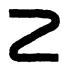
\includegraphics[keepaspectratio]{images/part001_a1e78629.jpg}}

注意，T 含于 \(\mu\) 的支集 S 与 g 的支集之交，但未必等于这一交。例如，若 X = R， \(\mu\) 是点 0 处的 Dirac 测度，且 \(g(x) = x\) ，则 \(g \cdot \mu = 0\) ，尽管 g 与 \(\mu\) 的支集之交退缩为点 0，因而是非空的。

推论. --- 为使测度 \(g \cdot \mu\) 为零，必须且只须 g 在 \(\mu\) 的支集上为零。

命题 11. --- 每个具紧支集的测度都是有界的。

因为 \(|\mu|\) 也是具紧支集的测度，故可只限于 \(\mu \geqslant 0\) 的情形；若 \(h\) 是 \(X\) 到 {[}0,1{]} 中的一个连续映射，具紧支集且在 \(\operatorname{Supp}(\mu)\) 上等于 1，则对每个函数 \(f \in \mathcal{K}(X; \mathbf{C})\) ，有 \(|f(x)| \leqslant \|f\|h(x)\) 在 \(\operatorname{Supp}(\mu)\) 上，因此（命题 8 的推论 2） \(\mu(|f|) \leqslant \mu(h)\|f\|\) ，这就证明了该命题（§1, No.~8）。

\subsection{点测度. 有限支集的测度}

命题 12. --- 设 \(a_i\) （ \(1 \leqslant i \leqslant n\) ）是局部紧空间 X 中互不相同的点。X 上每个支集含于诸 \(a_i\) 所成之集的测度都是诸测度 \(\varepsilon_{a_i}\) （ \(1 \leqslant i \leqslant n\) ）的一个线性组合。

因为这样的测度 \(\mu\) 对每个函数 \(f\in\mathcal{K}(\mathrm{X};\mathbf{C})\) （满足 \(n\) 个关系 \(f(a_{i})=0\) ）都为零（No.~3, 命题 8）；由于这些关系可写成 \(\varepsilon_{a_{i}}(f)=0\) ，故 \(\mu\) 是诸 \(\varepsilon_{a_{i}}\) 的线性组合（A, II, §7, No.~5, Th. 7 的推论 1）。

特别地，每个支集或为空集或退缩为单独一点 x 的测度都具有 \(\alpha\varepsilon_{x}\) 的形式，其中 \(\alpha\) 是一个复数；这样的测度称为点测度；于是每个支集为有限集的测度是点测度之和。

定理 1. --- 每个测度 \(\mu\) （局部紧空间 \(X\) 上的）都属于向量空间 \(V\) （由支集有限且含于 \(\operatorname{Supp}(\mu)\) 的测度构成）的淡闭包。

只需证明 \(\mu\) 与子空间 \(V^{\circ}\) （\(\mathcal{K}(X; \mathbf{C})\) 中与 \(V\) 正交的子空间）正交（TVS, II, §6, No.~3, Th. 1 的推论 2），也就是说，关系式 \(\langle f, \varepsilon_{a} \rangle = 0\) （其中 \(a\) 跑遍 \(\mu\) 的支集）蕴涵 \(\langle f, \mu \rangle = 0\) ；而这正是 No.~3 的命题 8。

推论 1. --- X 上的每个有界测度 \(\mu\) 都属于由支集有限、含于 \(\mu\) 的支集且范数 \(\leqslant \| \mu \|\) 的测度所构成的凸集 A 的淡闭包。此外，若 \(\nu\) 保持在 A 中而淡趋于 \(\mu\) ，则 \(\| \nu \|\) 趋于 \(\| \mu \|\) 。

为证第一个断言，只需证明测度 \(\mu\) 属于极集 \(A^{\circ}\) （A 在 \(\mathcal{K}(X;C)\) 中的极集）的极集（TVS, II, §6, No.~3, Th. 1 与 §8, No.~4）；这就是说，对 \(f \in \mathcal{K}(X;C)\) ，关系 \(|\langle f,\varepsilon_{a}\rangle| \leqslant 1/\|\mu\|\) 对一切 \(a \in \operatorname{Supp}(\mu)\) 成立蕴涵 \(|\langle f,\mu\rangle| \leqslant 1\) ；而这是 No.~3 命题 8 的推论 3 的推论。

为证第二个断言，我们注意

\[
\liminf _ {\nu \to \mu ,   \nu \in A} \| \nu \| \geqslant \| \mu \|
\]

因为函数 \(\nu \mapsto \| \nu \|\) 对淡拓扑是下半连续的（§1, No.~9, 命题 15 的推论 4），而结论由如下事实得出：按定义， \(\| \nu \| \leqslant \| \mu \|\) 对 \(\nu \in A\) 成立。

推论 2. --- 每个有界测度 \(\mu\) （\(X\) 上的）都属于由支集有限、含于 \(\mu\) 的支集且范数等于 \(\|\mu\|\) 的测度所成之集的淡闭包。

可以假设 \(\mu \neq 0\) 。设 \(V\) 是淡拓扑下 0 的一个开邻域；对每个 \(\varepsilon\) （满足 \(0 < \varepsilon < 1\) ），依据推论 1，存在一个测度 \(\nu_0\) ，其支集有限且含于 \(\operatorname{Supp}(\mu)\) ，并使 \(\nu_0 - \mu \in V\) 且 \(\| \mu \| \geqslant \| \nu_0 \| \geqslant (1 - \varepsilon) \| \mu \|\) 。令 \(\nu = (\| \mu \| / \| \nu_0 \|) \nu_0\) ，则有 \(\| \nu \| = \| \mu \|\) 且 \(\| \nu - \nu_0 \| \leqslant \| \mu \|\) ；因此对充分小的 \(\varepsilon\) 有 \(\nu - \mu \in V + V\) ，由此得结论。

推论 3. --- 每个有界正测度 \(\mu\) （\(X\) 上的）都属于由支集有限、含于 \(\mu\) 的支集且范数等于 \(\|\mu\|\) 的正测度所构成的凸集的淡闭包。

与推论 2 相同的推理表明，可以只限于证明 \(\mu\) 属于由支集有限、含于 \(\mathrm{Supp}(\mu)\) 且范数 \(\leqslant \| \mu \|\) 的正测度所构成的凸集 B 的淡闭包。同样，只需证明 \(\mu\) 属于 \(\mathbf{B}^{\circ}\) （即 B 在空间 \(\mathcal{K}(\mathbf{X};\mathbf{R})\) 中的极集）的极集（TVS, II, §6, No.~3, Th. 1）；这就是说，对 \(f\in \mathcal{K}(\mathbf{X};\mathbf{R})\) ，关系 \(\langle f,\varepsilon_a\rangle \geqslant -1 / \| \mu \|\) 对一切 \(a\in \mathrm{Supp}(\mu)\) 成立蕴涵 \(\langle f,\mu \rangle \geqslant -1\) ，而这是 No.~3 命题 8 的推论 2 的推论。

推论 4. --- 在空间 \(\mathcal{M}(\mathrm{X};\mathbf{C})\) 中，点测度所成之集对严格紧收敛拓扑是全的（§1, No.~10）。

在锥 \(\mathcal{M}_{+}(X)\) 上，严格紧收敛拓扑与淡拓扑相同（§1, No.~10, 命题 18），且 X 上的每个测度都可写成 \(\mu_{1}-\mu_{2}+i\mu_{3}-i\mu_{4}\) ，其中诸 \(\mu_{j}\ (1\leqslant j\leqslant4)\) 是正测度；因此结论由 Th. 1 得出。

命题 13. --- 设 \(\mu\) 是局部紧空间 \(X\) 上的一个测度。为使一点 \(x_0\) 属于 \(\operatorname{Supp}(\mu)\) ，必须且只须点测度 \(\varepsilon_{x_0}\) 属于测度 \(g \cdot \mu\) 所成之集的淡闭包，其中 \(g\) 跑遍满足 \(\| g \cdot \mu \| \leqslant 1\) 的具紧支集连续函数所成之集。

依据 No.~2 的命题 6，该条件显然是充分的。为证其必要性，设 \(x_0 \in \operatorname{Supp}(\mu)\) ；考虑有限个函数 \(f_k\) （ \(1 \leqslant k \leqslant n\) ，属于 \(\mathcal{K}(X; \mathbf{C})\) ）及任意一个数 \(\delta > 0\) ；我们要证明存在一个函数 \(g \in \mathcal{K}(X; \mathbf{C})\) ，使 \(\| g \cdot \mu \| \leqslant 1\) 且

\[
\left| f _ {k} \left(x _ {0}\right) - \mu \left(g f _ {k}\right) \right| \leqslant \delta
\]

对 \(1 \leqslant k \leqslant n\) 成立。设 U 是 \(x_0\) 的一个相对紧开邻域，使诸 \(f_k\) （ \(1 \leqslant k \leqslant n\) ）中每一个在 U 上的振幅 \(\leqslant \delta/2\) 。按假设，由于 \(x_0 \in \text{Supp}(\mu)\) ，存在一个函数 \(g_0 \in \mathcal{K}(X; \mathbf{C})\) ，其支集含于 U 且使 \(\mu(g_0) \neq 0\) ；测度 \(\nu = g_0 \cdot \mu\) 不为零，因为对每个在 U 上等于 1 的函数 \(f \in \mathcal{K}(X; \mathbf{C})\) ，有 \(\nu(f) = \mu(g_0) \neq 0\) 。此外， \(\nu\) 是有界的（No.~3, 命题 11）；

用标量乘 \(g_{0}\) ，可设 \(\|\nu\|=1\) 。在此条件下，令 \(\alpha_{k}=f_{k}(x_{0})\) ，则对 \(1\leqslant k\leqslant n\) 及每个函数 \(h\in\mathcal{K}(\mathrm{X};\mathbf{C})\) ，可写

\[
f _ {k} (x _ {0}) - \nu (f _ {k} h) = \alpha_ {k} (1 - \nu (h)) + \nu ((\alpha_ {k} - f _ {k}) h).
\]

由于 \(\nu\) 的支集在 U 中，可把它与其在 U 上的限制等同起来；于是假设 \(\| \nu \| = 1\) 蕴涵存在一个函数 \(h \in \mathcal{K}(\mathrm{X};\mathbf{C})\) ，其支集含于 U，使 \(\| h \| \leqslant 1\) 且 \(|\alpha_{k}(1 - \nu (h))| \leqslant \delta / 2\) 对 \(1 \leqslant k \leqslant n\) 成立。此外，U 的定义表明 \(|(\alpha_{k} - f_{k}(x))h(x)| \leqslant \delta / 2\) 对所有 \(x \in \mathrm{U}\) 成立；由于 \(\| \nu \| = 1\) 且 \(\operatorname{Supp}(\nu) \subset \mathrm{U}\) ，我们有 \(|\nu ((\alpha_{k} - f_{k})h)| \leqslant \delta / 2\) ，于是令 \(g = g_0h\) ，

\[
\left| f _ {k} \left(x _ {0}\right) - \mu \left(g f _ {k}\right) \right| \leqslant \delta \quad \text { for } 1 \leqslant k \leqslant n.
\]

这就证明了该命题，因为 \(\| g\cdot \mu \| = \| (g_0h)\cdot \mu \| \leqslant \| g_0\cdot \mu \| = 1\)

推论. --- 设 \(\mu\) 是 X 上的一个测度。为使 X 上的一个测度 \(\nu\) 属于测度 \(g \cdot \mu\) 所成之集（其中 \(g\) 跑遍 \(\mathcal{K}(X; \mathbf{C})\) ）的淡闭包，必须且只须 \(\operatorname{Supp}(\nu) \subset \operatorname{Supp}(\mu)\) 。

因为依据 No.~3 的命题 10，有 \(\operatorname{Supp}(g\cdot\mu)\subset\operatorname{Supp}(\mu)\) ；因此 \(g\cdot\mu\) 型测度的每个淡极限的支集也含于 \(\operatorname{Supp}(\mu)\) （No.~2, 命题 6）。反之，若 \(\operatorname{Supp}(\nu)\subset\operatorname{Supp}(\mu)\) ，则 \(\nu\) 是支集有限且含于 \(\operatorname{Supp}(\mu)\) 的测度的淡极限（Th. 1），因而由命题 13，它属于测度 \(g\cdot\mu\) 所成之集的淡闭包。

\subsection{离散测度}

命题 14. --- 为使测度 \(\mu\) （局部紧空间 \(X\) 上的）是离散测度（§1, No.~3, 例 I），必须且只须 \(\operatorname{Supp}(\mu)\) 是 \(X\) 的一个离散闭子空间。

设 \(\mu\) 是 X 上的一个离散测度，由质量 \(h(x) \neq 0\) （放在 X 的离散闭子空间 N 的各点 \(x\) 处）所定义；我们证明 \(\operatorname{Supp}(\mu) = \mathbf{N}\) 。对每个 \(a \in \mathbf{N}\) 及 \(a\) 的每个邻域 V，存在一个函数 \(f \in \mathcal{K}(\mathbf{X}; \mathbf{C})\) ，其支集含于 V，在点 \(a\) 处等于 1 而在 N 的其他点处等于 0，于是 \(\mu(f) = h(a) \neq 0\) 。另一方面，若 \(b \notin \mathbf{N}\) ，则存在 \(b\) 的一个不与 N 相交的邻域 W；于是对每个支集含于 W 的函数 \(g \in \mathcal{K}(\mathbf{X}; \mathbf{C})\) ，有 \(\mu(g) = 0\) ，这就证明 \(b \notin \operatorname{Supp}(\mu)\) 。

反之，设 \(\mu\) 是使 \(\operatorname{Supp}(\mu)\) 为 X 的离散闭子空间 N 的一个测度。对每个 \(a \in N\) ，存在 a 的一个不含 N 中异于 a 的点的开邻域 \(V_{a}\) ；因此 \(\mu\) 在 \(V_{a}\) 上的限制是支集为 \(\{a\}\) 的点测度（No.~2, 命题 5），从而（No.~4, 命题 12）具有 \(h(a)\varepsilon_{a}\) 的形式，其中 \(h(a)\neq0\) 。令 \(h(x)=0\) 在 \(\complement N\) 的各点处，并以 \(\nu\) 记由诸质量 \(h(x)\) 定义的测度，则局部化原理表明 \(\nu=\mu\) 。

由此可知，在离散空间 X 上，每个测度都是离散的。

\section{连续向量值函数的积分}

在本节中，X 恒表示一个局部紧空间，E 表示 R 或 C 上的一个局部凸空间。我们以 \(E'\) 表示 E 的对偶（E 上连续线性形式所成的空间），以 \(E'^{*}\) 表示 \(E'\) 的代数对偶（\(E'\) 上全体线性形式所成的空间）；对 \(z \in E\) ， \(z' \in E'\) ， \(z'^{*} \in E'^{*}\) ，我们写 \(\langle z, z' \rangle = z'(z)\) ， \(\langle z'^{*}, z' \rangle = z'^{*}(z')\) 。

回顾一下，若 E 是 Hausdorff 的，则 E 可等同于 \(E^{\prime*}\) 的一个线性子空间：把元素 \(z \in E\) 等同于线性形式 \(z' \mapsto \langle z, z' \rangle\) （\(E'\) 上的）；并且 \(E^{\prime*}\) 赋以弱拓扑 \(\sigma(E^{\prime*}, E')\) 后可典范地等同于赋以弱化拓扑 \(\sigma(E, E')\) 的 E 的完备化。

\subsection{向量值函数的积分的定义}

回顾一下，称 X 到 E 中的一个映射 \(\mathbf{f}\) 是弱连续的，如果对每个 \(\mathbf{z}' \in \mathrm{E}'\) ，映射 \(x \mapsto \langle \mathbf{f}(x), \mathbf{z}' \rangle\) （X 到 \(\mathbf{C}\) 中的；换言之即映射 \(\mathbf{z}' \circ \mathbf{f}\) ，也记作 \(\langle \mathbf{f}, \mathbf{z}' \rangle\) ）是连续的。我们称 X 到 E 中的映射 \(\mathbf{f}\) 是标量意义具有紧支集的，如果对每个 \(\mathbf{z}' \in \mathrm{E}'\) ，映射 \(x \mapsto \langle \mathbf{f}(x), \mathbf{z}' \rangle\) 具有紧支集。我们以 \(\widetilde{\mathcal{K}}(\mathrm{X};\mathrm{E})\) 表示 X 到 E 中的弱连续且标量意义具有紧支集的映射所成的空间；显然 \(\widetilde{\mathcal{K}}(\mathrm{X};\mathrm{E}) \supset \mathcal{K}(\mathrm{X};\mathrm{E})\) ，但这两个空间未必相同（见下面的例 2）；然而当 E 是有限维时它们相等。

注意，在弱连续（相应地，标量意义具有紧支集）函数的定义中，E 的拓扑仅通过对偶 \(E'\) 的中介而起作用；因此，当把 E 的拓扑换成任何使对偶相同的局部凸拓扑时，这些函数所成之集并不改变。

若 E 与 F 是一对对偶的向量空间，则应注意：说 X 到 E 中的映射对 \(\sigma(\mathrm{E},\mathrm{F})\) 连续与说它是弱连续的，二者含义相同。

设 \(\mathbf{f}\) 是 \(X\) 到 \(E\) 中的一个弱连续且标量意义具有紧支集的映射，并设 \(\mu\) 是 \(X\) 上的一个测度；对每个 \(\mathbf{z}' \in E'\) ，我们有 \(\mathbf{z}' \circ \mathbf{f} \in \mathcal{K}(X)\) ；令

\[
\varphi (\mathbf {z} ^ {\prime}) = \int \langle \mathbf {f} (x), \mathbf {z} ^ {\prime} \rangle d \mu (x) = \mu (\mathbf {z} ^ {\prime} \circ \mathbf {f}).
\]

显然 \(\varphi\) 是 \(\mathbf{E}'\) 上的一个线性形式，因而是 \(\mathbf{E}^{\prime*}\) 的一个元素。

定义 1. --- 对每个函数 \(\mathbf{f} \in \widetilde{\mathcal{K}}(\mathrm{X};\mathrm{E})\) ，我们把 \(\mathbf{f}\) 关于 \(\mu\) 的积分（记作 \(\int \mathbf{f} d\mu\) ，或 \(\int \mathbf{f}(x) d\mu(x)\) ，或 \(\int \mathbf{f}\mu\) ，或 \(\int \mathbf{f}(x)\mu(x)\) ）理解为 \(\mathrm{E}'^*\) 中由下式定义的元素：

\[
\left\langle \int \mathbf {f} d \mu , \mathbf {z} ^ {\prime} \right\rangle = \int \left\langle \mathbf {f}, \mathbf {z} ^ {\prime} \right\rangle d \mu \quad \text {for all} \mathbf {z} ^ {\prime} \in \mathrm{E} ^ {\prime}.\tag{1}
\]

注意，即使 E 是 Hausdorff 的且 \(\mathbf{f} \in \mathcal{K}(\mathrm{X};\mathrm{E})\) ，也未必有 \(\int f d\mu \in E\) （习题 1；参见 No.~3）。

例子. --- 1) 设 E 是 C 上有限维的 Hausdorff 空间，于是若 \((\mathbf{e}_{i})_{1\leqslant i\leqslant n}\) 是 E 的一个基，则映射

\[
\left(\xi_ {1}, \dots \xi_ {n}\right) \mapsto \sum_ {i = 1} ^ {n} \xi_ {i} \mathbf {e} _ {i}
\]

是 \(\mathbf{C}^n\) 到 \(\mathbf{E}\) 上的一个同构。于是我们知道 \(\mathbf{E}\) 上每个线性形式都是连续的，换言之， \(\mathbf{E}'\) 与 \(\mathbf{E}^*\) （\(\mathbf{E}\) 的代数对偶）相同，且 \(\mathbf{E}'^*\) 可典范地等同于 \(\mathbf{E}\) 。设 \((\mathbf{e}_i')_{1 \leqslant i \leqslant n}\) 是 \(\mathbf{E}'\) 中与 \((\mathbf{e}_i)\) 对偶的基；为使映射 \(\mathbf{f}\) （\(\mathbf{X}\) 到 \(\mathbf{E}\) 中的）是弱连续且标量意义具有紧支集的，必须且只须诸函数 \(f_i = \mathbf{e}_i' \circ \mathbf{f}\) 是具紧支集的连续函数；于是有 \(\mathbf{f}(x) = \sum_{i=1}^{n} f_i(x) \mathbf{e}_i\) 对所有 \(x \in \mathbf{X}\) 成立，且

\[
\int \mathbf {f} d \mu = \sum_ {i = 1} ^ {n} \mu (f _ {i}) \mathbf {e} _ {i}.
\]

\begin{enumerate}
\def\labelenumi{\arabic{enumi})}
\setcounter{enumi}{1}
\tightlist
\item
  取 E 为 X 上测度所成的空间 \(\mathcal{M}(\mathrm{X};\mathbf{C})\) ，赋以淡拓扑（ \(\S1\) , No.~9）；于是 E 的对偶 \(E'\) 可典范地等同于空间 \(\mathcal{K}(\mathrm{X};\mathbf{C})\) （TVS, II, \(\S6\) , No.~2, 命题 3）。X 到 E 中的映射 \(x \mapsto \varepsilon_{x}\) 是连续的（ \(\S1\) , No.~9, 命题 13），但当 X 不是紧时其支集不是紧的；然而它是标量意义具有紧支集的，因为对每个函数 \(f \in E'\) ，函数 \(x \mapsto \langle \varepsilon_x, f \rangle = f(x)\) 按定义具有紧支集。此外，
\end{enumerate}

\[
\int \left\langle \varepsilon_ {x}, f \right\rangle d \mu = \int f (x) d \mu (x) = \left\langle \mu , f \right\rangle
\]

对每个函数 \(f \in \mathcal{K}(\mathrm{X};\mathbf{C}) = \mathrm{E}'\) 成立，这就证明

\[
\int \varepsilon_ {x} d \mu (x) = \mu
\]

对 X 上的每个测度 \(\mu\) 成立。

\begin{enumerate}
\def\labelenumi{\arabic{enumi})}
\setcounter{enumi}{2}
\tightlist
\item
  若 \(\mathbf{E}\) 是 Hausdorff 的，则对每点 \(y \in \mathbf{X}\) 及每个函数 \(\mathbf{f} \in \widetilde{\mathcal{K}}(\mathbf{X};\mathbf{E})\) ，有
\end{enumerate}

\[
\int \mathbf {f} d \varepsilon_ {y} = \mathbf {f} (y)
\]

因为按定义 \(\int \langle \mathbf{f},\mathbf{z}^{\prime}\rangle d\varepsilon_{y} = \langle \mathbf{f}(y),\mathbf{z}^{\prime}\rangle\) 。

注. --- 1) 设 E 是一个局部凸空间，N 是 \(\{0\}\) 在 E 中的闭包，于是 \(E_{1} = E/N\) 是与 E 相伴的 Hausdorff 局部凸空间；我们知道对偶 \(E'\) 与 \(E_{1}'\) 相同；为使函数 f 属于 \(\widetilde{\mathcal{K}}(X;E)\) ，必须且只须 \(f_{1} = \pi \circ f\) （其中 \(\pi : E \to E_{1}\) 是典范同态）属于 \(\widetilde{\mathcal{K}}(X;E_{1})\) ，且此时 \(\int f d\mu = \int f_{1} d\mu\) 。因此可以只限于考虑 Hausdorff 局部凸空间。

\begin{enumerate}
\def\labelenumi{\arabic{enumi})}
\setcounter{enumi}{1}
\tightlist
\item
  设 E 是 C 上的一个局部凸空间， \(E_{0}\) 是 E 的底层 R 上局部凸空间；我们知道映射 \(z^{\prime} \mapsto Rz^{\prime}\) ——它把 E 上每个连续（复）线性形式 \(z^{\prime}\) 对应到连续（实）线性形式 \(z \mapsto R\langle z, z^{\prime} \rangle\) （\(E_{0}\) 上的）——是 \(E^{\prime}\) 到对偶 \(E_{0}^{\prime}\) （\(E_{0}\) 的）上的一个 R-同构（TVS, II, §8, No.~1）。类似地， \(E_{0}^{\prime *}\) （实向量空间 \(E_{0}^{\prime}\) 的代数对偶）可典范地等同于 \(E^{\prime *}\) （\(E^{\prime}\) 的代数对偶）的底层实空间。由此可知，若 \(\mu\) 是一个实测度而 f 是 \(\widetilde{\mathcal{K}}(X;E)\) 中的一个映射，则当把 f 看作取值于 \(E_{0}\) ，并把两个成员中出现的典范双线性型分别看作：第一个成员相对于 \(E_{0}^{\prime}\) 与 \(E_{0}^{\prime *}\) 之间的对偶，第二个成员相对于 \(E_{0}\) 与 \(E_{0}^{\prime}\) 之间的对偶时，公式 (1) 仍然成立。
\end{enumerate}

\subsection{向量积分的性质}

命题 1. --- 映射

\[
(\mathbf {f}, \mu) \mapsto \int \mathbf {f} d \mu
\]

（\(\widetilde{\mathcal{K}} (\mathrm{X};\mathrm{E})\times \mathcal{M}(\mathrm{X};\mathbf{C})\) 到 \(\mathrm{E}^{\prime *}\) 中的）是双线性的。

该命题由 No.~1 的定义 1 立即得出。

设 \(\mathbf{u}\) 是 \(\mathrm{E}\) 到一个局部凸空间 \(\mathrm{F}\) 中的一个连续线性映射；我们知道转置 \(^t\mathbf{u}\) 是 \(\mathrm{F}'\) （\(\mathrm{F}\) 的对偶）到 \(\mathrm{E}'\) （\(\mathrm{E}\) 的对偶）中的一个线性映射；我们以 \(^{tt}\mathbf{u}\) 记 \(\mathrm{E}^{\prime *} \to \mathrm{F}^{\prime *}\) 的映射，即 \(^t\mathbf{u}\) 的（代数意义的）转置；当 \(\mathrm{E}\) 与 \(\mathrm{F}\) 都是 Hausdorff 的且分别典范地等同于 \(\mathrm{E}^{\prime *}\) 与 \(\mathrm{F}^{\prime *}\) 的子空间时， \(^{tt}\mathbf{u}\) 是映射 \(\mathbf{u}\) 的延拓。在这些记号下：

命题 2. --- 设 u 是 E 到一个局部凸空间 F 中的一个连续线性映射；对每个函数 \(\mathbf{f} \in \widetilde{\mathcal{K}}(\mathrm{X};\mathrm{E})\) ，函数 \(\mathbf{u} \circ \mathbf{f}\) 属于 \(\widetilde{\mathcal{K}}(\mathrm{X};\mathrm{F})\) ，且

\[
\int \mathbf {u} (\mathbf {f} (x)) d \mu (x) = ^ {t t} \mathbf {u} \left(\int \mathbf {f} (x) d \mu (x)\right).\tag{2}
\]

对每个连续线性形式 \(z^{\prime} \in F^{\prime}\) ，有 \(z^{\prime} \circ u \circ f = y^{\prime} \circ f\) （令 \(y^{\prime} = z^{\prime} \circ u = {}^{t}u(z^{\prime}) \in E^{\prime}\) ），由此得第一个断言；此外，对所有 \(z^{\prime} \in F^{\prime}\) ，

\[
\begin{array}{r l} \left\langle \int (\mathbf {u} \circ \mathbf {f}) d \mu , \mathbf {z} ^ {\prime} \right\rangle & = \int \langle \mathbf {u} \circ \mathbf {f}, \mathbf {z} ^ {\prime} \rangle d \mu = \int \langle \mathbf {f}, ^ {t} \mathbf {u} (\mathbf {z} ^ {\prime}) \rangle d \mu \\ & = \left\langle \int \mathbf {f} d \mu , ^ {t} \mathbf {u} (\mathbf {z} ^ {\prime}) \right\rangle = \left\langle {} ^ {t t} \mathbf {u} \left(\int \mathbf {f} d \mu\right), \mathbf {z} ^ {\prime} \right\rangle , \end{array}
\]

由此得公式 (2)。

命题 3. --- 对每个函数 \(g \in \mathcal{C}(\mathrm{X};\mathbf{C})\) 及每个函数 \(\mathbf{f} \in \widetilde{\mathcal{K}}(\mathrm{X};\mathrm{E})\) ，函数 \(g\mathbf{f}\) 属于 \(\widetilde{\mathcal{K}}(\mathrm{X};\mathrm{E})\) ，且

\[
\int \mathbf {f} d (g \cdot \mu) = \int \mathbf {f} g d \mu .\tag{3}
\]

事实上，对每个 \(z^{\prime} \in E^{\prime}\) ， \(\langle gf, z^{\prime} \rangle = g\langle f, z^{\prime} \rangle\) ，由此得第一个断言；此外，

\[
\begin{array}{r l} \left\langle \int \mathbf {f} d (g \cdot \mu), \mathbf {z} ^ {\prime} \right\rangle & = \int \langle \mathbf {f}, \mathbf {z} ^ {\prime} \rangle d (g \cdot \mu) = \int g \langle \mathbf {f}, \mathbf {z} ^ {\prime} \rangle d \mu \\ & = \int \langle g \mathbf {f}, \mathbf {z} ^ {\prime} \rangle d \mu = \left\langle \int g \mathbf {f} d \mu , \mathbf {z} ^ {\prime} \right\rangle , \end{array}
\]

由此得 (3)。

命题 4. --- 设 \(\mu\) 是 X 上的一个正测度，S 是其支集，f 是 \(\widetilde{\mathcal{K}}(\mathrm{X};\mathrm{E})\) 中的一个函数。设 E 是 Hausdorff 的，并给空间 \(\mathrm{E}^{\prime*}\) 赋以弱拓扑 \(\sigma(\mathrm{E}^{\prime*},\mathrm{E}^{\prime})\) 。

\begin{enumerate}
\def\labelenumi{(\roman{enumi})}
\item
  积分 \(\int \mathbf{f}d\mu\) 属于 C ，即 \(\mathrm{E}^{\prime *}\) 中由 \(\mathbf{f}(\mathrm{S})\) 生成的凸锥的闭包。
\item
  若 \(\mu\) 有界，则积分 \(\int \mathbf{f} d\mu\) 属于集 \(\| \mu \| \cdot D\) ，其中 \(D\) 是 \(\mathbf{f}(S)\) 在 \(\mathrm{E}'^*\) 中的闭凸包。
\end{enumerate}

若 \(\mathrm{E}\) 是复的，我们给 \(\mathrm{E}\) 赋以其底层实向量空间结构，如前所述，这并不改变公式 (1)。

\begin{enumerate}
\def\labelenumi{(\roman{enumi})}
\tightlist
\item
  我们知道 C 是 \(E^{\prime*}\) 中包含 \(\mathbf{f}(\mathrm{S})\) 且由过 0 的闭超平面确定的闭半空间之交；因此只需证明，对 \(z^{\prime} \in E^{\prime}\) ，关系 \(\langle\mathbf{f}(x), \mathbf{z}^{\prime}\rangle \geqslant 0\) 对一切 \(x \in S\) 成立蕴涵
\end{enumerate}

\[
\left\langle \int \mathbf {f} d \mu , \mathbf {z} ^ {\prime} \right\rangle \geqslant 0;
\]

但由于

\[
\left\langle \int \mathbf {f} d \mu , \mathbf {z} ^ {\prime} \right\rangle = \int \left\langle \mathbf {f}, \mathbf {z} ^ {\prime} \right\rangle d \mu ,
\]

这由 §2, No.~3, 命题 8 的推论 2 得出。

\begin{enumerate}
\def\labelenumi{(\roman{enumi})}
\setcounter{enumi}{1}
\tightlist
\item
  我们知道 D 是 \(E^{\prime*}\) 中包含 \(\mathbf{f}(S)\) 的闭半空间之交；因此只需证明，对 \(z^{\prime} \in E^{\prime}\) ，关系 \(\langle\mathbf{f}(x), \mathbf{z}^{\prime}\rangle \leqslant a\) 对一切 \(x \in S\) 成立蕴涵
\end{enumerate}

\[
\left\langle \int \mathbf {f} d \mu , \mathbf {z} ^ {\prime} \right\rangle \leqslant a \| \mu \|;
\]

而这由 §2, No.~3, 命题 8 的推论 3 得出。

推论. --- 设 \(\mu\) 是 X 上的一个正测度，f 是属于 \(\mathcal{K}(\mathrm{X};\mathrm{E})\) 的一个映射，D 是 \(\mathbf{f}(\mathrm{X})\) 在 \(\mathrm{E}'^*\) 中的闭凸包。则存在一个数 \(a > 0\) 使 \(\int \mathbf{f} d\mu \in a \cdot \mathrm{D}\) 。

若 \(\nu\) 是 \(X\) 上的任一测度，则存在数 \(a_1, a_2, a_3, a_4 > 0\) 使 \(\int \mathbf{f} d\nu \in a_1\mathrm{D} - a_2\mathrm{D} + ia_3\mathrm{D} - ia_4\mathrm{D}\) 。

先设 \(\mu\) 是正的；按假设，f 的支集 K 是紧的；若 \(\nu\) 是 \(\mu\) 在 K 的一个相对紧开邻域上的限制，则 \(\nu\) 有界，且由命题 4, (ii)， \(\int f d\mu = \int f d\nu \in \|\nu\| \cdot D\) 。第二个结果由此得出，因为任何复测度都可写成 \(\mu_{1} - \mu_{2} + i\mu_{3} - i\mu_{4}\) ，其中诸 \(\mu_{j}\) 是正测度。

命题 5. --- 设空间 X 是紧的，f 是 X 到一个 Hausdorff 局部凸空间 E 中的一个连续映射。 \(\mathbf{f}(\mathbf{X})\) 在 \(E^{\prime*}\) 中（对 \(\sigma(E^{\prime*}, E^{\prime})\) ）的闭凸包等于向量 \(\int f d\mu\) （对 X 上总质量为 1 的一切正测度 \(\mu\) 所取）所成之集。

设 C 是 \(\mathbf{f}(\mathbf{X})\) 在 \(E^{\prime*}\) 中的闭凸包；由于 \(\mathbf{f}(\mathbf{X})\) 是紧的且 \(E^{\prime*}\) 是完备的，故 C 是紧的。我们已经知道（命题 4），

\(\int \mathbf{f}d\mu \in \mathbb{C}\) 对属于 X 上总质量等于 1 的正测度所成凸集 H 的每个测度 \(\mu\) 成立。另一方面，H 对淡拓扑是凸的且紧的（§1, No.~9, 命题 15 的推论 3），且是质量为 1、支集有限的正测度所成凸集 \(\mathrm{H}_0\) 的（对该拓扑的）闭包（§2, No.~4, Th. 1 的推论 3）。现在， \(\mathrm{H}_0\) 在映射 \(\mu \mapsto \int \mathbf{f}d\mu\) 下的像是凸包 \(\mathrm{C}_0\) ，即 \(\mathbf{f}(\mathbf{X})\) 在 \(\mathrm{E}'^*\) 中的凸包。另一方面，这一映射对 \(\mathcal{M}(\mathrm{X};\mathbf{C})\) 上的淡拓扑与拓扑 \(\sigma (\mathrm{E}^{\prime *},\mathrm{E}^{\prime})\) （\(\mathrm{E}'^*\) 上的）是连续的，因为按定义 \(\langle \int \mathbf{f}d\mu ,\mathbf{z}'\rangle = \int \langle \mathbf{f},\mathbf{z}'\rangle d\mu\) ；于是 \(\mathrm{H} = \overline{\mathrm{H}}_0\) 的像是一个包含 \(\mathrm{C}_0\) 且含于 C 的紧凸集；由于 \(\mathrm{C} = \overline{\mathrm{C}}_0\) ，这个像等于 C。

命题 6. --- 对 X 到一个 Hausdorff 局部凸空间 E 中的每个具紧支集的连续映射 f、E 上每个连续半范数 q 及 X 上的每个测度 \(\mu\) （使 \(\int f d\mu \in E\) ），

\[
q \left(\int \mathbf {f} d \mu\right) \leqslant \int (q \circ \mathbf {f}) d | \mu |.\tag{4}
\]

设 D 是 \(z \in E\) （\(q(\mathbf{z}) \leqslant 1\) ）所成之集；D 是闭的、凸的且包含 0，因此 \(D = D^{\circ\circ}\) （TVS, II, §6, No.~3, Th. 1 的推论 3）。因此只需证明，对每个 \(z' \in D^{\circ}\) ，

\[
\left| \left\langle \int \mathbf {f} d \mu , \mathbf {z} ^ {\prime} \right\rangle \right| \leqslant \int (q \circ \mathbf {f}) d | \mu |;
\]

由于

\[
\left\langle \int \mathbf {f} d \mu , \mathbf {z} ^ {\prime} \right\rangle = \int \left\langle \mathbf {f}, \mathbf {z} ^ {\prime} \right\rangle d \mu ,
\]

且由于按 \(D^{\circ}\) 的定义，

\[
| \langle \mathbf {f} (x), \mathbf {z} ^ {\prime} \rangle | \leqslant q (\mathbf {f} (x))
\]

对所有 \(x \in \mathbf{X}\) 成立，故所欲证的不等式由 §1, No.~6 的不等式 (13) 得出。

\subsection{积分属于 E 的判据}

命题 7. --- 设 E 是一个 Hausdorff 局部凸空间，且 \(\mathbf{f} \in \mathcal{K}(\mathrm{X};\mathrm{E})\) 。若 \(\mathbf{f}(\mathrm{X})\) 含于 E 的一个完备凸子集 A，则 \(\int \mathbf{f} d\mu \in \mathbf{E}\) 。

设 K 是 f 的支集，按假设它是紧的。由于 f 在 X - K 上为零， \(\mathbf{f}(X)\) 等于 \(\mathbf{f}(K)\) 或 \(\mathbf{f}(K) \cup \{0\}\) ，因 f 连续且 E 是 Hausdorff 的，故它是紧的；于是 \(\mathbf{f}(X)\) 在 E 中的闭凸包 C 是预紧的（对由 E 的一致结构诱导的一致结构而言）（TVS, II, §4, No.~1, 命题 3）。但由于 C 是完备空间 A 的一个闭子集，故 C 是完备的从而是紧的；更有甚者，C 对弱化拓扑 \(\sigma(\mathrm{E}, \mathrm{E}')\) 是紧的；由于该拓扑是由 \(\sigma(\mathrm{E}'*, \mathrm{E}')\) 诱导的，故 C 也是 \(\mathbf{f}(X)\) 在 \(E'\) 中对拓扑 \(\sigma(\mathrm{E}'*, \mathrm{E}')\) 的闭凸包；于是证明由 No.~2 命题 4 的推论完成。

推论 1. --- 设 E 是一个 Hausdorff 局部凸空间；对每个函数 \(\mathbf{f} \in \mathcal{K}(\mathrm{X};\mathrm{E})\) ， \(\int \mathbf{f} d\mu\) 属于 E 的完备化 \(\widehat{\mathbf{E}}\) 。

由于 E 与 \(\widehat{E}\) 的对偶相同，只需把 f 看作取值于 \(\widehat{E}\) 而应用命题 7。

推论 2. --- 若 E 是一个拟完备的 Hausdorff 局部凸空间，则 \(\int \mathbf{f} d\mu \in \mathrm{E}\) 对每个函数 \(\mathbf{f} \in \mathcal{K}(\mathrm{X};\mathrm{E})\) 成立。

如命题 7 证明开头所指出的， \(\mathbf{f}(\mathrm{X})\) 是紧的，且其在 E 中的闭凸包 C 是预紧的，从而是有界的；但由于集 C 是闭的且有界，按假设它是完备的，于是只需应用命题 7。

在 Ch. VI, §1, No.~2 中，我们将看到 \(\int \mathbf{f} d\mu\) 属于 E 的其他判据，它们特别适用于 \(\widetilde{\mathcal{K}}(\mathrm{X};\mathrm{E})\) 中的函数，而不仅限于 \(\mathcal{K}(\mathrm{X};\mathrm{E})\) 中的函数。

命题 7 的推论 2 可应用于下述两种情形：\(1^{\circ}\) E 是 Banach 空间；\(2^{\circ}\) E 是某个桶式 Hausdorff 局部凸空间 G 的对偶，且 E 赋以某个 S-拓扑，其中 S 是 G 由有界子集组成的一个覆盖（TVS, III, §4, No.~2, Th. 1 的推论 4）。例如，当 E 是 Banach 空间的弱对偶，或是赋以淡拓扑的测度空间 \(\mathcal{M}(\mathrm{Y};\mathbf{C})\) 时，可以应用命题 7 的推论 2。

若 \(\mathbf{X} = \mathbf{R}\) ， \(\mu\) 是 \(\mathbf{R}\) 上的 Lebesgue 测度，且 \(\mathrm{E}\) 是 Banach 空间，则积分 \(\int \mathbf{f} d\mu\) （ \(\mathcal{K}(\mathrm{X};\mathrm{E})\) 中函数的）不是别的，正是在

\[
\int_ {- \infty} ^ {+ \infty} \mathbf {f} (x) d x
\]

中定义的积分，即 FRV, II, §2, No.~1 中的积分；这由公式 (1) 及 FRV, I, §1, No.~2, 命题 2 的推论得出。

\subsection{积分的连续性质}

命题 8. --- 设 E 是 Hausdorff 的；设 \(\mu\) 是 X 上的一个测度。映射 \(\mathbf{f} \mapsto \int \mathbf{f} d\mu\) （ \(\mathcal{K}(\mathrm{X};\mathbf{E})\) 到 \(\widehat{\mathbf{E}}\) 中的；No.~3, 命题 7 的推论 1）是唯一的连续线性映射 \(\Phi\) ，它满足 \(\Phi(g \cdot \mathbf{a}) = \mu(g) \cdot \mathbf{a}\) 对每个向量 \(\mathbf{a} \in \mathbf{E}\) 及每个函数 \(g \in \mathcal{K}(\mathrm{X};\mathbf{C})\) 。

为证映射 \(f \mapsto \int f d\mu\) 的连续性，只需证明它在 \(\mathcal{K}(X, K; E)\) 上的限制对 X 的每个紧子集 K 都是连续的（TVS, II, §4, No.~4, 命题 5）。我们注意，若 E 的拓扑由半范数族 \((q_{\alpha})\) 定义，则 \(\mathcal{K}(X, K; E)\) 的拓扑由半范数族

\[
p _ {\alpha} (\mathbf {f}) = \sup _ {x \in K} q _ {\alpha} \bigl (\mathbf {f} (x) \bigr).
\]

定义。现在，设 h 是 X 到 \([0,1]\) 中的一个连续映射，具紧支集且在 K 上 \(h(x)=1\) ；由 No.~2 的命题 6，对每个函数 \(\mathbf{f}\in\mathcal{K}(\mathrm{X},\mathrm{K};\mathrm{E})\) 有

\[
q _ {\alpha} \left(\int \mathbf {f} d \mu\right) = q _ {\alpha} \left(\int h \mathbf {f} d \mu\right) \leqslant \int h (x) q _ {\alpha} (\mathbf {f} (x)) d | \mu | (x) \leqslant | \mu | (h) \cdot p _ {\alpha} (\mathbf {f})
\]

（诸 \(q_{\alpha}\) 已连续地延拓到 \(\widehat{\mathbf{E}}\) 上），这就证明了 \(\mathbf{f} \mapsto \int \mathbf{f} d\mu\) 的连续性。另一方面，按陈述中的记号，

\[
\int \left(g (x) \cdot {\bf a}\right) d \mu (x) = \mu (g) \cdot {\bf a}
\]

这依据 No.~1 的例 1 及 No.~2 的命题 2 应用于典范单射 \(\mathbf{C} \cdot \mathbf{a} \to \mathrm{E}\) 而得。此外， \(\mathcal{K}(\mathrm{X};\mathrm{E})\) 中由线性组合 \(\sum_{i} g_i \cdot \mathbf{a}_i\) （其中 \(\mathbf{a}_i \in \mathrm{E}\) ， \(g_i \in \mathcal{K}(\mathrm{X};\mathbf{C})\) ）所构成的子空间在 \(\mathcal{K}(\mathrm{X};\mathrm{E})\) 中稠密（§1, No.~2, 命题 5），这就完成了证明。

命题 9. --- 设 E 是 Hausdorff 的；设 f 是 X 到 E 中的一个具紧支集的连续映射。当空间 \(\mathcal{M}(\mathrm{X};\mathbf{C})\) 赋以严格紧收敛拓扑（§1, No.~10）时，映射 \(\mu \mapsto \int \mathbf{f} d\mu\) （ \(\mathcal{M}(\mathrm{X};\mathbf{C})\) 到 \(\widehat{\mathrm{E}}\) 中的）是唯一的连续线性映射 \(\Psi\) ，它满足 \(\Psi(\varepsilon_x) = \mathbf{f}(x)\) 对所有 \(x \in \mathrm{X}\) 。

对每个 \(\mathbf{z}' \in \mathrm{E}'\) ，

\[
\left\langle \int \mathbf {f} d \varepsilon_ {x}, \mathbf {z} ^ {\prime} \right\rangle = \int (\mathbf {z} ^ {\prime} \circ \mathbf {f}) d \varepsilon_ {x} = \mathbf {z} ^ {\prime} (\mathbf {f} (x)) = \langle \mathbf {f} (x), \mathbf {z} ^ {\prime} \rangle ,
\]

由此得 \(\int \mathbf{f} d\varepsilon_x = \mathbf{f}(x)\) 。此外我们知道，点测度所成之集在 \(\mathcal{M}(\mathrm{X};\mathbf{C})\) 中对严格紧收敛拓扑是全的（§2, No.~4, Th. 1 的推论 4）。于是问题归结为证明线性映射 \(u: \mu \mapsto \int \mathbf{f} d\mu\) 的连续性。为此，考虑线性映射 \(v: \mathbf{z}' \mapsto \langle \mathbf{f}, \mathbf{z}' \rangle\) （ \(\mathrm{E}'\) 到 \(\mathcal{K}(\mathrm{X};\mathbf{C})\) 中的），并证明 \(v\) 把一个等度连续子集 H （ \(\mathrm{E}'\) 的）映入 \(\mathcal{K}(\mathrm{X};\mathbf{C})\) 的一个严格紧子集中。因为若 K 是 \(\mathbf{f}\) 的支集，则诸函数 \(\langle \mathbf{f}, \mathbf{z}' \rangle\) （对 \(\mathbf{z}' \in \mathrm{H}\) ）的支集都含于 K；另一方面，这些函数构成一个等度连续集，且对每个 \(x \in \mathrm{X}\) ，诸 \(\mathbf{z}'(\mathbf{f}(x))\) 所成之集是有界的；于是我们的断言由 Ascoli 定理得出（GT, X, §2, No.~5, Th. 2 的推论 3）。现在，由 No.~1 的公式 (1) 可知， \(u\) 不是别的，正是 \(\mathcal{M}(\mathrm{X};\mathbf{C})\) 上的转置 \(^t v\) （代数意义的）的限制；因此其连续性由前述事实得出（TVS, IV, §1, No.~3, 命题 6）。

推论. --- 在命题 9 的假设与记号下，映射 \(\mu \mapsto \int \mathbf{f} d\mu\) 在正测度所成之集 \(\mathcal{M}_{+}(\mathrm{X})\) 上、或在 \(\mathcal{M}(\mathrm{X};\mathbf{C})\) 的一个淡有界子集 B 上的限制是淡连续的。

因为由 §1, No.~10 的命题 17 与 18 可知，在 \(\mathcal{M}_{+}(X)\) 上或在 B 上，由严格紧收敛拓扑诱导的拓扑与由淡拓扑诱导的拓扑相同。

\pandocbounded{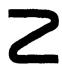
\includegraphics[keepaspectratio]{images/part001_df9b2198.jpg}}

然而，映射 \(\mu \mapsto \int \mathbf{f}d\mu\) 在整个 \(\mathcal{M}(\mathrm{X};\mathbf{C})\) 上对淡拓扑未必连续（习题 2）。

\section{测度的乘积}

\subsection{两个测度的乘积}

定理 1. --- 设 X 与 Y 是两个局部紧空间， \(\lambda\) 是 X 上的一个测度， \(\mu\) 是 Y 上的一个测度；则存在唯一的测度 \(\nu\) （X \(\times\) Y 上的），使得对每个函数 \(g \in \mathcal{K}(\mathrm{X};\mathbf{C})\) 及每个函数 \(h \in \mathcal{K}(\mathrm{Y};\mathbf{C})\) ，

\[
\int g (x) h (y) d \nu (x, y) = \left(\int g (x) d \lambda (x)\right) \left(\int h (y) d \mu (y)\right).\tag{1}
\]

引理 1. --- 设 X 与 Y 是两个局部紧空间，K（相应地 L）是 X（相应地 Y）的一个紧子集。

\begin{enumerate}
\def\labelenumi{(\roman{enumi})}
\tightlist
\item
  典范双射在 \(\mathcal{K}(\mathrm{X}\times \mathrm{Y},\mathrm{K}\times \mathrm{L};\mathbf{C})\) 上的限制
\end{enumerate}

\[
\omega : \mathcal {F} (\mathrm{X} \times \mathrm{Y}; \mathbf {C}) \rightarrow \mathcal {F} \bigl (\mathrm{X}; \mathcal {F} (\mathrm{Y}; \mathbf {C}) \bigr)
\]

（S, R, §4, No.~14）是 Banach 空间 \(\mathcal{K}(\mathrm{X}\times\mathrm{Y},\mathrm{K}\times\mathrm{L};\mathbf{C})\) 到 Banach 空间 \(\mathcal{K}(\mathrm{X},\mathrm{K};\mathcal{K}(\mathrm{Y},\mathrm{L};\mathbf{C}))\) 上的一个等距。

\begin{enumerate}
\def\labelenumi{(\roman{enumi})}
\setcounter{enumi}{1}
\tightlist
\item
  向量空间 \(\mathcal{K}(\mathrm{X},\mathrm{K};\mathbf{C})\otimes_{\mathbf{C}}\mathcal{K}(\mathrm{Y},\mathrm{L};\mathbf{C})\) （典范地等同于 \(\mathcal{K}(\mathrm{X}\times \mathrm{Y},\mathrm{K}\times \mathrm{L};\mathbf{C})\) 的一个子空间；A, II, §7, No.~7, 命题 15 的推论之后的注记）在这个 Banach 空间中稠密。
\end{enumerate}

\(\omega\) 下 \(\mathcal{K}(X\times Y,K\times L;C)\) 的像含于 \(\mathcal{K}(X,K;\mathcal{K}(Y,L;C))\) ，这是直接的。反之，若 u 是 X 到 \(\mathcal{K}(Y,L;C)\) 中的一个连续映射，其支集含于 K，则映射 \((x,y)\mapsto\mathbf{u}(x)(y)\) （ \(X\times Y\) 到 C 中的）是连续的且支集含于 \(K\times L\) ，因此 \(\omega\) 在 \(\mathcal{K}(X\times Y,K\times L;C)\) 上的限制是此空间到 \(\mathcal{K}(X,K;\mathcal{K}(Y,L;C))\) 上的一个双射；这一限制是 Banach 空间等距这一事实由关系式

\[
\sup _ {(x, y) \in \mathrm{K} \times \mathrm{L}} | f (x, y) | = \sup _ {x \in \mathrm{K}} \left(\sup _ {y \in \mathrm{L}} | f (x, y) |\right).
\]

得出。这就证明了 (i)；另一方面，在 \(\omega\) 下，

\[
\mathcal {K} (\mathrm{X}, \mathrm{K}; \mathbf {C}) \otimes_ {\mathbf {C}} \mathcal {K} (\mathrm{Y}, \mathrm{L}; \mathbf {C})
\]

（等同于 \(\mathcal{K}(\mathrm{X}\times \mathrm{Y},\mathrm{K}\times \mathrm{L};\mathbf{C})\) 的一个子空间）的像仍是空间 \(\mathcal{K}(\mathrm{X},\mathrm{K};\mathbf{C})\otimes_{\mathbf{C}}\mathcal{K}(\mathrm{Y},\mathrm{L};\mathbf{C})\) ，不过这次是典范地等同于 X 到 \(\mathcal{K}(\mathrm{Y},\mathrm{L};\mathbf{C})\) 中的映射所成的一个空间（A, II, §7, No.~7, 命题 15 的推论）；而 \(\mathcal{K}(\mathrm{X},\mathrm{K};\mathcal{K}(\mathrm{Y},\mathrm{L};\mathbf{C}))\) 的这一子空间已知在后一空间中稠密（§1, No.~2, 命题 5），于是 (ii) 的结论由 \(\omega\) 的这一限制是拓扑同构这一事实得出。

引理证毕之后，我们现在注意， \(X \times Y\) 的每个紧子集都含于某个乘积 \(K \times L\) 之中，其中 K（相应地 L）是 X（相应地 Y）的一个紧子集。于是由引理 1, (ii) 可知，子空间 \(\mathcal{K}(X; \mathbf{C}) \otimes_{\mathbf{C}} \mathcal{K}(Y; \mathbf{C})\) 在 \(\mathcal{K}(X \times Y; \mathbf{C})\) 中稠密；由于关系式 (1) 也可写成 \(\nu(g \otimes h) = \lambda(g)\mu(h)\) （对 \(g \in \mathcal{K}(X; \mathbf{C})\) ， \(h \in \mathcal{K}(Y; \mathbf{C})\) ），故 \(\nu\) 的唯一性立即得出。为证 \(\nu\) 的存在性，我们将使用下述引理：

引理 2. --- 在引理 1 的记号下，对每个函数 \(f \in \mathcal{K}(\mathrm{X} \times \mathrm{Y}, \mathrm{K} \times \mathrm{L}; \mathbf{C})\) ，函数

\[
y \mapsto h (y) = \int f (x, y) d \lambda (x)\tag{2}
\]

属于 \(\mathcal{K}(\mathrm{Y},\mathrm{L};\mathbf{C})\)

对每个函数 \(\mathbf{u} \in \mathcal{K}(\mathrm{X};\mathcal{K}(\mathrm{Y},\mathrm{L};\mathbf{C}))\) ，积分 \(\int \mathbf{u}(x)d\lambda (x)\) 属于 \(\mathcal{K}(\mathrm{Y},\mathrm{L};\mathbf{C})\) ，因为后者是 Banach 空间（ \(\S 3\) , No.~3, 命题 7 的推论 1）；而对 \(\mathbf{u} = \omega(f)\) 及每个 \(y \in \mathrm{Y}\) ，

\[
\left\langle \int \mathbf {u} (x) d \lambda (x), \varepsilon_ {y} \right\rangle = \int \mathbf {u} (x) (y) d \lambda (x) = \int f (x, y) d \lambda (x),
\]

由此得该引理。

于是，对每个函数 \(f \in \mathcal{K}(\mathrm{X} \times \mathrm{Y}; \mathbf{C})\) ，考虑数 \(\nu(f) = \mu\left(\int f(x, y) d\lambda(x)\right)\) （出于记号的滥用，我们也把它写作 \(\int d\mu(y) \int f(x, y) d\lambda(x)\) ）；若 K（相应地 L）是 X（相应地 Y）的一个紧子集，则存在一个数 \(a_{K}\) （相应地 \(b_{L}\) ），使得对每个函数 \(g \in \mathcal{K}(\mathrm{X}, \mathrm{K}; \mathbf{C})\) （相应地 \(h \in \mathcal{K}(\mathrm{Y}, \mathrm{L}; \mathbf{C})\) ）有 \(|\lambda(g)| \leqslant a_{\mathrm{K}} \|g\|\) （相应地 \(|\mu(h)| \leqslant b_{\mathrm{L}} \|h\|\) ）。由此可知，对每个函数 \(f \in \mathcal{K}(\mathrm{X} \times \mathrm{Y}, \mathrm{K} \times \mathrm{L}; \mathbf{C})\) ，

\[
\left| \int f (x, y) d \lambda (x) \right| \leqslant a _ {K} \| f \|
\]

对每个 \(y \in Y\) 成立，由此得 \(|\nu(f)| \leqslant a_{K}b_{L}\|f\|\) 。于是线性形式 \(\nu\) （ \(\mathcal{K}(X \times Y; \mathbf{C})\) 上的）是 \(X \times Y\) 上的一个测度，它显然满足 (1)，这就完成了 Th. 1 的证明。

定义 1. --- 给定分别定义在两个局部紧空间 X、Y 上的两个测度 \(\lambda\) 、 \(\mu\) ，我们把 \(\lambda\) 与 \(\mu\) 的乘积测度定义为唯一的测度 \(\nu\) （ \(X \times Y\) 上的），它对每个函数 \(g \in \mathcal{K}(X; \mathbf{C})\) 及每个函数 \(h \in \mathcal{K}(Y; \mathbf{C})\) 满足关系式 (1)。

在 Th. 1 的证明中，X 与 Y 两空间的地位可以互换；把 \(Y \times X\) 与 \(X \times Y\) 典范地等同起来，我们便在 \(X \times Y\) 上定义了测度

\[
f \mapsto \int d \lambda (x) \int f (x, y) d \mu (y)
\]

它仍满足条件 (1)。于是我们证明了下述定理：

定理 2. --- 设 \(\lambda\) 、 \(\mu\) 是分别定义在两个局部紧空间 \(X\) 、 \(Y\) 上的两个测度。对每个函数 \(f\) （ \(\mathcal{K}(X \times Y; \mathbf{C})\) 中的），\(f\) 关于乘积测度 \(\nu\) （\(\lambda\) 与 \(\mu\) 的乘积）的积分的值为

\[
\begin{array}{c} \int f (x, y) d \nu (x, y) = \int d \lambda (x) \int f (x, y) d \mu (y) \\ = \int d \mu (y) \int f (x, y) d \lambda (x). \end{array}\tag{3}
\]

由于最后的公式，f 关于乘积测度 \(\nu\) 的积分通常记作 \(\iint f d\lambda d\mu\) ，或 \(\iint f d\mu d\lambda\) ，或 \(\iint f \lambda \mu\) ，或 \(\iint f \mu \lambda\) ，或 \(\iint f(x, y) d\lambda(x) d\mu(y)\) ，或 \(\iint f(x, y) d\mu(y) d\lambda(x)\) ，或 \(\iint f(x, y) \lambda(x)\mu(y)\) ，或 \(\iint f(x, y) \mu(y)\lambda(x)\) ；称它为 f 关于 \(\lambda\) 与 \(\mu\) 的二重积分。采用这一记号，公式 (3) 可写成

\[
\begin{array}{c} \iint f (x, y) d \lambda (x) d \mu (y) = \int d \lambda (x) \int f (x, y) d \mu (y) \\ = \int d \mu (y) \int f (x, y) d \lambda (x). \end{array}\tag{4}
\]

公式 (3) 表明，若 \(\lambda\) 与 \(\mu\) 是实（相应地，正）测度，则乘积测度 \(\nu\) 是实（相应地，正）测度。

例子. --- 1) Dirac 测度 \(\varepsilon_{x}\) （ \(x \in X\) ）与 \(\varepsilon_{y}\) （ \(y \in Y\) ）的乘积测度是 Dirac 测度 \(\varepsilon_{(x,y)}\) 。

\begin{enumerate}
\def\labelenumi{\arabic{enumi})}
\setcounter{enumi}{1}
\tightlist
\item
  取 \(\mathbf{X} = \mathbf{Y} = \mathbf{R}\) ，并取 \(\lambda\) 与 \(\mu\) 为 \(\mathbf{R}\) 上的 Lebesgue 测度（§1, No.~3）；其乘积称为 \(\mathbf{R}^2\) 上的 Lebesgue 测度；函数 \(f \in \mathcal{K}(\mathbf{R}^2; \mathbf{C})\) 关于该测度的积分记作 \(\iint f(x, y) dx dy\) 或 \(\iint f(x, y) dy dx\) ；公式 (4) 对在紧矩形 \([a, b] \times [c, d]\) 之外为零的函数给出公式
\end{enumerate}

\[
\int_ {c} ^ {d} d y \int_ {a} ^ {b} f (x, y) d x = \int_ {a} ^ {b} d x \int_ {c} ^ {d} f (x, y) d y
\]

这已在 FRV, II, §3, No.~6 中证明。

由于 \(\mathbf{R}\) 上的 Lebesgue 测度在每个平移下不变（§1, No.~3），立即得出 \(\mathbf{R}^2\) 上的 Lebesgue 测度在 \(\mathbf{R}^2\) 的每个平移下不变。

注. --- 设 E 是一个 Hausdorff 局部凸空间，f 是 \(\mathcal{K}(X \times Y; E)\) 中的一个映射，使得 \(\mathbf{f}(X \times Y)\) 含于 E 的一个完备凸子集 C。于是对每个 \(y \in Y\) ，积分 \(\mathbf{h}(y) = \int \mathbf{f}(x, y) d\lambda(x)\) 属于 E（§3, No.~3, 命题 7）；此外，函数 h 属于 \(\widetilde{\mathcal{K}}(Y; E)\) ：因为对每个 \(z' \in E'\) 有

\[
\langle \mathbf {h} (y), \mathbf {z} ^ {\prime} \rangle = \int \langle \mathbf {f} (x, y), \mathbf {z} ^ {\prime} \rangle d \lambda (x),
\]

因而由引理 2， \(y \mapsto \langle \mathbf{h}(y), \mathbf{z}' \rangle\) 属于 \(\mathcal{K}(\mathrm{Y}; \mathbf{C})\) 。于是积分 \(\int h d\mu\) 有定义（且先验地属于 \(E'^{*}\) ）；我们证明

\[
\begin{array}{r l} \iint \mathbf {f} (x, y) d \lambda (x) d \mu (y) & = \int d \mu (y) \int \mathbf {f} (x, y) d \lambda (x) \\ & = \int d \lambda (x) \int \mathbf {f} (x, y) d \mu (y), \end{array}\tag{5}
\]

从而把公式 (4) 加以推广。事实上，对每个 \(\mathbf{z}' \in \mathrm{E}'\) 有

\[
\begin{array}{r l} \left\langle \iint \mathbf {f} d \lambda d \mu , \mathbf {z} ^ {\prime} \right\rangle & = \iint \langle \mathbf {f}, \mathbf {z} ^ {\prime} \rangle d \lambda d \mu = \int d \mu \int \langle \mathbf {f}, \mathbf {z} ^ {\prime} \rangle d \lambda \\ & = \int \left\langle \int \mathbf {f} d \lambda , \mathbf {z} ^ {\prime} \right\rangle d \mu = \left\langle \int d \mu \int \mathbf {f} d \lambda , \mathbf {z} ^ {\prime} \right\rangle \end{array}
\]

这是依据 (4)，由此得 (5)。

\subsection{乘积测度的性质}

若 \(\lambda\) （相应地 \(\mu\) ）是 X（相应地 Y）上的一个测度，而 \(\nu\) 是 \(\lambda\) 与 \(\mu\) 的乘积测度，则 \(\nu\) 在 \(\mathcal{K}(X;C)\otimes_{\mathbf{C}}\mathcal{K}(Y;C)\) 上的限制不是别的，正是张量积 \(\lambda\otimes\mu\) ，即两个线性形式 \(\lambda\) 与 \(\mu\) 的张量积（A, II, §3, No.~2），因为 No.~1 的关系式 (1) 可写成

\[
\langle g \otimes h, \nu \rangle = \langle g, \lambda \rangle \langle h, \mu \rangle = \langle g \otimes h, \lambda \otimes \mu \rangle
\]

对所有 \(g \in \mathcal{K}(X; \mathbf{C})\) 及 \(h \in \mathcal{K}(Y; \mathbf{C})\) 成立。出于记号的滥用，我们也用 \(\lambda \otimes \mu\) 表示乘积测度 \(\nu\) （而不仅是它在 \(\mathcal{K}(X; \mathbf{C}) \otimes_{\mathbf{C}} \mathcal{K}(Y; \mathbf{C})\) （ \(\mathcal{K}(X \times Y; \mathbf{C})\) 的稠密子空间）上的限制）。

映射 \((\lambda, \mu) \mapsto \lambda \otimes \mu\) （ \(\mathcal{M}(\mathrm{X}; \mathbf{C}) \times \mathcal{M}(\mathrm{Y}; \mathbf{C})\) 到 \(\mathcal{M}(\mathrm{X} \times \mathrm{Y}; \mathbf{C})\) 中的）显然是双线性的，这依据 No.~1 的公式 (3)。

命题 1. --- 设 \(\lambda\) 是 X 上的一个测度， \(\mu\) 是 Y 上的一个测度；若 \(g \in \mathcal{C}(\mathrm{X};\mathbf{C})\) ， \(h \in \mathcal{C}(\mathrm{Y};\mathbf{C})\) ，则

\[
(g \cdot \lambda) \otimes (h \cdot \mu) = (g \otimes h) \cdot (\lambda \otimes \mu).\tag{6}
\]

对每个函数 \(f \in \mathcal{K}(\mathrm{X} \times \mathrm{Y}; \mathbf{C})\) ，依据 No.~1 的公式 (3)，有

\[
\begin{array}{c} \langle f, (g \otimes h) \cdot (\lambda \otimes \mu) \rangle = \int d \lambda (x) \int f (x, y) g (x) h (y) d \mu (y) \\ = \int g (x) d \lambda (x) \int f (x, y) h (y) d \mu (y), \end{array}
\]

这就证明了公式 (6)。

命题 2. --- 乘积 \(\lambda \otimes \mu\) 的支集等于 \(\lambda\) 的支集与 \(\mu\) 的支集之积。

我们首先注意，关系式 \(\lambda \otimes \mu = 0\) 蕴涵测度 \(\lambda, \mu\) 之一为零（A, II, §7, No.~7, 命题 16, (ii)）。另一方面，若 U（相应地 V）是 X（相应地 Y）中的开集，则 \(\lambda\otimes\mu\) 在乘积 \(U\times V\) 上的限制是 \(\lambda\) 在 U 上的限制与 \(\mu\) 在 V 上的限制之积，这由 No.~1 的 Th. 1 及测度在开集上的限制的定义（§2, No.~1）得出。于是由此可知，为使 \(\lambda\otimes\mu\) 在 \(U\times V\) 上的限制为零，必须且只须 \(\lambda\) 在 U 上的限制或 \(\mu\) 在 V 上的限制为零，再考虑到测度支集的定义（§2, No.~2），这就证明了该命题。

命题 3. --- 设 \(\lambda \in \mathcal{M}(\mathrm{X};\mathbf{C})\) ， \(\mu \in \mathcal{M}(\mathrm{Y};\mathbf{C})\) 。则

\[
| \lambda \otimes \mu | = | \lambda | \otimes | \mu |.\tag{7}
\]

设 \(f \in \mathcal{K}_{+}(\mathrm{X} \times \mathrm{Y})\) ， \(g \in \mathcal{K}(\mathrm{X} \times \mathrm{Y}; \mathbf{C})\) 满足 \(|g| \leqslant f\) ；我们有（§1, No.~6, 公式 (13)）

\[
\begin{array}{r l} | \langle g, \lambda \otimes \mu \rangle | = & \left| \int d \lambda (x) \int g (x, y)   d \mu (y) \right| \\ & \leqslant \int d | \lambda | (x) \int | g (x, y) |   d | \mu | (y) \\ & = \langle | g |, | \lambda | \otimes | \mu | \rangle \leqslant \langle f, | \lambda | \otimes | \mu | \rangle . \end{array}
\]

由此得 \(\langle f, |\lambda \otimes \mu| \rangle \leqslant \langle f, |\lambda| \otimes |\mu| \rangle\) ，于是

\[
| \lambda \otimes \mu | \leqslant | \lambda | \otimes | \mu |.\tag{8}
\]

另一方面，设 \(u \in \mathcal{K}_{+}(\mathrm{X})\) ， \(v \in \mathcal{K}_{+}(\mathrm{Y})\) 。对每个 \(\varepsilon > 0\) ，存在 \(u_{1} \in \mathcal{K}(\mathrm{X};\mathbf{C})\) ， \(v_{1} \in \mathcal{K}(\mathrm{Y};\mathbf{C})\) ，使 \(|u_{1}| \leqslant u\) ， \(|v_{1}| \leqslant v\) ，且

\[
| \langle u _ {1}, \lambda \rangle | \geqslant \langle u, | \lambda | \rangle - \varepsilon , \quad | \langle v _ {1}, \mu \rangle | \geqslant \langle v, | \mu | \rangle - \varepsilon
\]

（§1, No.~6）。由此得 \(|u_1 \otimes v_1| \leqslant u \otimes v\) ，且

\[
\begin{array}{c} \langle u \otimes v, | \lambda \otimes \mu | \rangle \geqslant | \langle u _ {1} \otimes v _ {1}, \lambda \otimes \mu \rangle | = | \langle u _ {1}, \lambda \rangle \langle v _ {1}, \mu \rangle | \\ \geqslant (\langle u, | \lambda | \rangle - \varepsilon) (\langle v, | \mu | \rangle - \varepsilon). \end{array}
\]

由于 \(\varepsilon\) 是任意的，我们推出

\[
\langle u \otimes v, | \lambda \otimes \mu | \rangle \geqslant \langle u, | \lambda | \rangle \langle v, | \mu | \rangle = \langle u \otimes v, | \lambda | \otimes | \mu | \rangle .
\]

把 (8) 考虑在内，我们便得

\[
\langle u \otimes v, | \lambda \otimes \mu | \rangle = \langle u \otimes v, | \lambda | \otimes | \mu | \rangle .
\]

由于 \(\mathcal{K}(\mathrm{X};\mathbf{C})\) （相应地 \(\mathcal{K}(\mathrm{Y};\mathbf{C})\) ）中的每个函数都是 \(\mathcal{K}_{+}(\mathrm{X})\) （相应地 \(\mathcal{K}_{+}(\mathrm{Y})\) ）中函数的线性组合，前面的公式对 \(u\in\mathcal{K}(\mathrm{X};\mathbf{C})\) 与 \(v\in\mathcal{K}(\mathrm{Y};\mathbf{C})\) 仍成立；于是该命题由 \(\mathcal{K}(\mathrm{X};\mathbf{C})\otimes_{\mathbf{C}}\mathcal{K}(\mathrm{Y};\mathbf{C})\) 在 \(\mathcal{K}(\mathrm{X}\times\mathrm{Y};\mathbf{C})\) 中稠密这一事实得出。

推论. --- 设 \(\lambda \in \mathcal{M}(\mathrm{X};\mathbf{R})\) ， \(\mu \in \mathcal{M}(\mathrm{Y};\mathbf{R})\) 。则

\[
\left\{ \begin{array}{l} (\lambda \otimes \mu) ^ {+} = \lambda^ {+} \otimes \mu^ {+} + \lambda^ {-} \otimes \mu^ {-}, \\ (\lambda \otimes \mu) ^ {-} = \lambda^ {+} \otimes \mu^ {-} + \lambda^ {-} \otimes \mu^ {+}. \end{array} \right.\tag{9}
\]

因为依据命题 3，

\[
\begin{array}{r l} & {(\lambda \otimes \mu) ^ {+} = \frac {1}{2} \big (\lambda \otimes \mu + | \lambda | \otimes | \mu | \big)} \\ & {\qquad = \frac {1}{2} \big ((\lambda^ {+} - \lambda^ {-}) \otimes (\mu^ {+} - \mu^ {-}) + (\lambda^ {+} + \lambda^ {-}) \otimes (\mu^ {+} + \mu^ {-}) \big)} \\ & {\qquad = \lambda^ {+} \otimes \mu^ {+} + \lambda^ {-} \otimes \mu^ {-}.} \end{array}
\]

对 \((\lambda \otimes \mu)^{-}\) 的论证是类似的。

命题 4. --- 设 \(\lambda \in \mathcal{M}(\mathrm{X};\mathbf{C})\) ， \(\mu \in \mathcal{M}(\mathrm{Y};\mathbf{C})\) 。则

\[
\| \lambda \otimes \mu \| = \| \lambda \| \cdot \| \mu \|,\tag{10}
\]

并约定每当一个因子为 0 而另一因子为 +∞ 时，第二成员换成 0。特别地，若 λ 与 μ 有界，则 λ⊗μ 有界。

由上面的命题 3 及 §1, No.~8, 命题 10 的推论 1，可以只限于 \(\lambda\) 与 \(\mu\) 是正测度的情形。若 \(\lambda = 0\) 或 \(\mu = 0\) ，结果是平凡的；故设 \(\lambda \neq 0\) 且 \(\mu \neq 0\) 。先证明 \(\| \lambda \otimes \mu \| \leqslant \| \lambda \| \cdot \| \mu \|\) 。可设 \(\lambda\) 与 \(\mu\) 有界。对每个 \(f \in \mathcal{K}_+(\mathrm{X} \times \mathrm{Y})\) ，

\[
\langle f, \lambda \otimes \mu \rangle = \int d \lambda (x) \int f (x, y) d \mu (y)
\]

且

\[
\int f (x, y) d \mu (y) \leqslant \| f \| \cdot \| \mu \|
\]

对每个 \(x\in \mathbf{X}\) 成立，因此

\[
\langle f, \lambda \otimes \mu \rangle \leqslant \| f \| \cdot \| \lambda \| \cdot \| \mu \|,
\]

这就证明了我们的断言。另一方面，设

\[
\alpha <   \| \lambda \|, \beta <   \| \mu \|
\]

为两个实数 \(\geqslant 0\) 。存在 \(g\in \mathcal{K}_{+}(\mathrm{X})\) ， \(h\in \mathcal{K}_{+}(\mathrm{Y})\) ，使

\[
\| g \| \leqslant 1, \| h \| \leqslant 1, \lambda (g) \geqslant \alpha , \mu (h) \geqslant \beta .
\]

于是 \(g \otimes h \in \mathcal{K}_{+}(X \times Y)\) ， \(\| g \otimes h \| \leqslant 1\) ，且 \(\langle g \otimes h, \lambda \otimes \mu \rangle \geqslant \alpha \beta\) ；因此 \(\| \lambda \otimes \mu \| \geqslant \alpha \beta\) ，最终得 \(\| \lambda \otimes \mu \| \geqslant \| \lambda \| \cdot \| \mu \|\) ，这就完成了证明。

\subsection{乘积测度的连续性}

命题 5. --- 对每个测度 \(\lambda_0 \in \mathcal{M}(\mathrm{X};\mathbf{C})\) ，映射 \(\mu \mapsto \lambda_0 \otimes \mu\) （ \(\mathcal{M}(\mathrm{Y};\mathbf{C})\) 到 \(\mathcal{M}(\mathrm{X} \times \mathrm{Y};\mathbf{C})\) 中的）是淡连续的。

对每个函数 \(f \in \mathcal{K}(\mathrm{X} \times \mathrm{Y}; \mathbf{C})\) ，我们知道函数 \(h(y) = \int f(x, y) d\lambda_0(x)\) 属于 \(\mathcal{K}(\mathrm{Y}; \mathbf{C})\) （No.~1, 引理 2），且 \(\langle f, \lambda_0 \otimes \mu \rangle = \langle h, \mu \rangle\) ，由此得该命题。

命题 6. --- 当 \(\mathcal{M}(\mathrm{X};\mathbf{C})\) 、 \(\mathcal{M}(\mathrm{Y};\mathbf{C})\) 与 \(\mathcal{M}(\mathrm{X}\times\mathrm{Y};\mathbf{C})\) 都赋以严格紧收敛拓扑（§1, No.~10）时，双线性映射 \((\lambda,\mu)\mapsto\lambda\otimes\mu\) （ \(\mathcal{M}(\mathrm{X};\mathbf{C})\times\mathcal{M}(\mathrm{Y};\mathbf{C})\) 到 \(\mathcal{M}(\mathrm{X}\times\mathrm{Y};\mathbf{C})\) 中的）对 \(\mathcal{M}(\mathrm{X};\mathbf{C})\) 与 \(\mathcal{M}(\mathrm{Y};\mathbf{C})\) 的淡有界子集全体是亚连续的（TVS, III, §5, No.~3）。

设 \(K \subset X\) ， \(L \subset Y\) 是两个紧集，A 是 \(\mathcal{K}(X \times Y, K \times L; C)\) 的一个紧子集，B 是 \(\mathcal{M}(X; C)\) 的一个淡有界闭子集；已知 B 是淡紧的（§1, No.~9, 命题 15），因而对严格紧收敛拓扑也是紧的（§1, No.~10, 命题 17）。另一方面，Banach 空间 \(\mathcal{K}(X \times Y, K \times L; C)\) 等距同构于 \(\mathcal{K}(X, K; \mathcal{K}(Y, L; C))\) （No.~1, 引理 1）；映射 \(\varphi\) （ \(\mathcal{K}(X, K; \mathcal{K}(Y, L; C)) \times \mathcal{M}(X; C)\) 到 \(\mathcal{K}(Y, L; C)\) 中的）——使 \(\varphi(g, \lambda)\) 为由 \(h(y) = \int g(x, y) d\lambda(x)\) 定义的函数 h——依据 §3, No.~4 的命题 8 与 9 是分别连续的。由于 \(\mathcal{K}(X, K; \mathcal{K}(Y, L; C))\) 是桶式的，由此可知映射 \(\varphi\) 相对于 \(\mathcal{M}(X; C)\) 的淡有界子集是亚连续的（TVS, III, §5, No.~3, 命题 6）；因此这一映射在 \(A \times B\) 上的限制是连续的（同处，命题 4）。于是 \(A \times B\) 在这一映射下的像 C 是 Banach 空间 \(\mathcal{K}(Y, L; C)\) 的一个紧子集。而 C 不是别的，正是函数 \(h(y) = \int f(x, y) d\lambda(x)\) （当 f 跑遍 A 且 \(\lambda\) 跑遍 B 时）所成之集；于是依据 No.~1 的公式 (3)，条件 \(\lambda \in B\) 与 \(\mu \in C^{\circ}\) 蕴涵 \(\lambda \otimes \mu \in A^{\circ}\) 。鉴于严格紧收敛拓扑的定义，这就证明了该命题（TVS, III, §5, No.~3, 定义 2）。

\pandocbounded{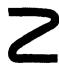
\includegraphics[keepaspectratio]{images/part001_f639fdbe.jpg}}

当把严格紧收敛拓扑换成淡拓扑时，命题 6 的结论不再成立（习题 2 c)）。然而，若 B（相应地 C）是 \(\mathcal{M}(\mathrm{X};\mathbf{C})\) （相应地 \(\mathcal{M}(\mathrm{Y};\mathbf{C})\) ）的一个淡有界子集，则 \(\mathrm{B}\times \mathrm{C}\) 在映射 \((\lambda ,\mu)\mapsto \lambda \otimes \mu\) 下的像在 \(\mathcal{M}(\mathrm{X}\times \mathrm{Y};\mathbf{C})\) 中是淡有界的，因而这一映射在 \(\mathrm{B}\times \mathrm{C}\) 上的限制是淡连续的，这依据命题 6、 §1, No.~10 的命题 17 以及 TVS, III, §5, No.~3 的命题 4（参见习题 3）。

\subsection{有限个测度的乘积}

设 \(X_{i}\) （ \(1 \leqslant i \leqslant n\) ）是 \(n\) 个局部紧空间， \(X = \prod_{i=1}^{n} X_{i}\) 是它们的乘积。形如

\[
\left(x _ {1}, x _ {2}, \dots , x _ {n}\right) \mapsto f _ {1} \left(x _ {1}\right) f _ {2} \left(x _ {2}\right) \dots f _ {n} \left(x _ {n}\right),
\]

（其中 \(f_{i} \in \mathcal{K}(\mathrm{X}_{i};\mathbf{C})\) ， \(1 \leqslant i \leqslant n\) ）的复函数的线性组合所成之集可典范地等同于张量积 \(\bigotimes_{i=1}^{n} \mathcal{K}(\mathrm{X}_{i};\mathbf{C})\) ，且由 No.~1 的引理 1（对 \(n\) 用归纳法）可知，这一张量积在 \(\mathcal{K}(\mathrm{X};\mathbf{C})\) 中稠密。

现在设 \(\mu_{i}\) 是 \(X_{i}\) （ \(1 \leqslant i \leqslant n\) ）上的一个测度；则在 X 上存在唯一的测度 \(\nu\) ，使得对 \(f_{i} \in \mathcal{K}(X_{i}; \mathbf{C})\) （ \(1 \leqslant i \leqslant n\) ），

\[
\left\langle f _ {1} \otimes f _ {2} \otimes \dots \otimes f _ {n}, \nu \right\rangle = \prod_ {i = 1} ^ {n} \left\langle f _ {i}, \mu_ {i} \right\rangle .\tag{11}
\]

因为若这一测度存在，则由前所述它是唯一的。另一方面，设 \(\nu = \mu_{1} \otimes \mu_{2} \otimes \cdots \otimes \mu_{n}\) 是由递归关系

\[
\mu_ {1} \otimes \mu_ {2} \otimes \dots \otimes \mu_ {n} = (\mu_ {1} \otimes \mu_ {2} \otimes \dots \otimes \mu_ {n - 1}) \otimes \mu_ {n}.
\]

在 X 上定义的测度。由 No.~1 的公式 (1) 及这一定义（对 n 用归纳法）可知 \(\nu\) 满足 (11)；称它为诸测度 \(\mu_{i}\) （ \(1 \leqslant i \leqslant n\) ）的乘积测度，并仍记作 \(\bigotimes_{i=1}^{n} \mu_{i}\) 。关系式 (11) 也可写成

\[
\left\langle f _ {1} \otimes f _ {2} \otimes \dots \otimes f _ {n}, \mu_ {1} \otimes \mu_ {2} \otimes \dots \otimes \mu_ {n} \right\rangle = \prod_ {i = 1} ^ {n} \left\langle f _ {i}, \mu_ {i} \right\rangle .\tag{12}
\]

命题 7（《测度乘积的结合律》）. --- 设 \((\mathbf{I}_k)_{1 \leqslant k \leqslant r}\) 是区间 \([1, n]\) （ \(\mathbf{N}\) 中的）的一个分割；则

\[
\bigotimes_ {k = 1} ^ {r} \left(\bigotimes_ {i \in I _ {k}} \mu_ {i}\right) = \bigotimes_ {i = 1} ^ {n} \mu_ {i}\tag{13}
\]

因为由 (12)，这两个测度对 \(\bigotimes_ {i = 1} ^ {n} \mathcal{K}(X_{i}; \mathbf{C})\) 中的每个函数取值相同。

函数 \(f \in \mathcal{K}(\mathbf{X};\mathbf{C})\) 关于乘积测度的积分记作

\[
\int f d \mu_ {1} d \mu_ {2} \dots d \mu_ {n},
\]

或

\[
\iint \ldots \int f d \mu_ {1} d \mu_ {2} \ldots d \mu_ {n}
\]

或

\[
\int f (\mu_ {1} \otimes \dots \otimes \mu_ {n})
\]

或

\[
\iint \dots \int f (x _ {1}, x _ {2}, \dots , x _ {n}) d \mu_ {1} (x _ {1}) d \mu_ {2} (x _ {2}) \dots d \mu_ {n} (x _ {n})
\]

或

\[
\iint \dots \int f (x _ {1}, x _ {2}, \dots , x _ {n}) \mu_ {1} (x _ {1}) \mu_ {2} (x _ {2}) \dots \mu_ {n} (x _ {n})
\]

（带 n 个积分号 \(\int\) ）；称它为 n 阶多重积分或 n 重积分。依据测度乘积的结合律及积分换序定理（No.~1, Th. 2），对每个置换 \(\sigma\) （ \([1,n]\) 的），有

\[
\iint \dots \int f d \mu_ {1} d \mu_ {2} \dots d \mu_ {n} = \int d \mu_ {\sigma (1)} \int d \mu_ {\sigma (2)} \dots \int f d \mu_ {\sigma (n)}.\tag{14}
\]

积分记号和公式 (14) 可以以明显的方式推广到函数 \(\mathbf{f} \in \mathcal{K}(\mathrm{X};\mathrm{E})\) （取值于 Hausdorff 局部凸空间 E 中、且 \(\mathbf{f}(\mathrm{X})\) 含于 E 的一个完备凸子集中的）。把 No. 2 与 No. 3 中关于两个测度的乘积的结果推广到任意有限个测度的乘积，这一工作留给读者。

特别地， \(\mathbf{R}^n\) 上的 Lebesgue 测度称为 \(n\) 个与 \(\mathbf{R}\) 上的 Lebesgue 测度相同的测度的乘积；满足前述条件的函数 \(\mathbf{f} \in \mathcal{K}(\mathbf{R}^n; \mathbf{E})\) 的积分记作

\[
\iint \dots \int \mathbf {f} (x _ {1}, x _ {2}, \dots , x _ {n}) d x _ {1} d x _ {2} \dots d x _ {n}
\]

并且等于

\[
\int_ {- \infty} ^ {+ \infty} d x _ {1} \int_ {- \infty} ^ {+ \infty} d x _ {2} \dots \int_ {- \infty} ^ {+ \infty} \mathbf {f} (x _ {1}, x _ {2}, \dots , x _ {n}) d x _ {n}.
\]

\(R^{n}\) 上的 Lebesgue 测度在每个平移下不变。
